\documentclass[11pt]{article}
\usepackage[margin=1in]{geometry}
\usepackage[T1]{fontenc}
\usepackage{lmodern,microtype}
\usepackage{graphicx,booktabs}
\usepackage{amsmath,amssymb,xcolor,listings,seqsplit}
\usepackage{tikz,enumitem,float,fancyhdr}
\usepackage[hidelinks]{hyperref}
% Shared visual system for every TikZ figure in this report.
% Colours are sampled from repo/layout.png, the annotated layout image that
% ships with the puzzle; see figures/src/palette.py for the measurement.
\usetikzlibrary{arrows.meta,positioning,calc,fit,backgrounds,shapes.geometric,
  decorations.pathreplacing,patterns}

\definecolor{figink}{HTML}{172033}     % body ink
\definecolor{figsoft}{HTML}{5B6472}    % secondary text
\definecolor{figaccent}{HTML}{3157A4}  % structure, arrows, frames
\definecolor{figblue}{HTML}{2196F3}    % layout.png: routing
\definecolor{figviolet}{HTML}{B388FF}  % layout.png: straps
\definecolor{figorange}{HTML}{FF8C1A}  % layout.png: vertical bars
\definecolor{figmagenta}{HTML}{E040E0} % layout.png: fine routes
\definecolor{figgold}{HTML}{C9A227}    % layout.png: local interconnect
\definecolor{figgreen}{HTML}{0A7D33}   % layout.png: output labels; used for
                                       % verified facts and final results
% The layout violet is a fill colour: as a hairline stroke or as small text it
% reads as grey. This is the same hue carried toward the ink so that clock
% wires and clock labels stay legible at figure sizes.
\definecolor{figclkline}{HTML}{7B52C4}
\definecolor{figrule}{HTML}{B9C0CC}    % muted outlines
\definecolor{figmute}{HTML}{F1F4F8}    % muted fills
\definecolor{figwash}{HTML}{EEF3FC}    % pale accent wash

% Narrow boxes hyphenate badly at this size, and a broken word costs more
% legibility than a ragged edge saves.
\newcommand{\fignohyphen}{\hyphenchar\font=-1 \hyphenpenalty=10000
  \exhyphenpenalty=10000 \tolerance=3000 \emergencystretch=3em}

% A card: eyebrow, title, body, hairline, and a monospace footer pinned to the
% bottom edge. Keeping the footer inside the frame stops the artefact names
% floating loose underneath, and a fixed height keeps a row of cards even.
% #1 name  #2 (x,y) of the top-left corner  #3 width/cm  #4 height/cm
% #5 style  #6 eyebrow  #7 title  #8 body  #9 footer
% The footer is anchored to the bottom edge and grows upward, so a two- or
% three-line footer stays inside the frame instead of spilling past it, and the
% hairline is placed from the footer's own top edge rather than a guessed offset.
\newcommand{\figcard}[9]{%
  \node[#5, anchor=north west, minimum width=#3cm, minimum height=#4cm,
        inner sep=0pt] (#1) at #2 {};
  \node[ftag, anchor=north west] at ($(#1.north west)+(0.22,-0.13)$) {#6};
  \node[figfont, anchor=north west, font=\sffamily\scriptsize\bfseries]
    at ($(#1.north west)+(0.22,-0.42)$) {#7};
  \node[figfont, anchor=north west, align=left,
        text width={\dimexpr #3cm-0.44cm}]
    at ($(#1.north west)+(0.22,-0.76)$) {\fignohyphen #8};
  \node[fmonosoft, anchor=south west, align=left,
        text width={\dimexpr #3cm-0.44cm}]
    (#1-foot) at ($(#1.south west)+(0.22,0.14)$) {#9};
  \draw[figrule, line width=0.4pt]
    ($(#1-foot.north west)+(0,0.10)$) -- ($(#1-foot.north east)+(0,0.10)$);
}

\tikzset{
  % applies inside every node's own text group, where it still governs how
  % lines are broken
  every node/.append style={execute at begin node=\fignohyphen},
  figfont/.style={font=\sffamily\scriptsize, text=figink},
  % a plain content box
  fbox/.style={figfont, draw=figaccent, fill=white, rounded corners=2pt,
    line width=0.5pt, align=center, inner sep=4pt},
  % a stage in a pipeline: title line plus supporting lines
  fstage/.style={fbox, fill=figwash, align=left, text width=#1},
  fstage/.default=3.1cm,
  % something established by evidence
  fgood/.style={fbox, draw=figgreen, fill=figgreen!5},
  % something taken on trust from outside the file
  ftrust/.style={fbox, draw=figorange, fill=figorange!6},
  % de-emphasised context
  fmuted/.style={figfont, draw=figrule, fill=figmute, rounded corners=2pt,
    line width=0.4pt, align=center, inner sep=3.5pt, text=figsoft},
  % arrows
  fflow/.style={-{Latex[length=2.1mm,width=1.5mm]}, draw=figaccent,
    line width=0.6pt},
  fthin/.style={-{Latex[length=1.6mm,width=1.2mm]}, draw=figsoft,
    line width=0.4pt},
  fdep/.style={draw=figsoft, line width=0.4pt, dash pattern=on 1.6pt off 1.4pt},
  % labels
  ftag/.style={font=\sffamily\tiny, text=figsoft, inner sep=1.5pt},
  fmono/.style={font=\ttfamily\tiny, text=figink, inner sep=1pt},
  fmonosoft/.style={font=\ttfamily\tiny, text=figsoft, inner sep=1pt},
  fhead/.style={font=\sffamily\scriptsize\bfseries, text=figaccent},
  %
  % ---- signal roles -----------------------------------------------------
  % One colour per role, used the same way in every schematic figure, so a
  % reader who learns the key once can carry it between diagrams:
  %   data      routing blue    the value being computed or carried
  %   clock     violet          when state advances, never a data term
  %   enable    magenta         whether this edge captures anything
  %   reset     orange          the asynchronous override
  % Green stays reserved for checked facts and final results. Captions identify
  % the smaller subset checked against genuinely independent evidence.
  fdata/.style={-{Latex[length=2.1mm,width=1.5mm]}, draw=figblue,
    line width=0.9pt},
  fclk/.style={-{Latex[length=2.1mm,width=1.5mm]}, draw=figclkline,
    line width=0.9pt},
  fen/.style={-{Latex[length=2.1mm,width=1.5mm]}, draw=figmagenta,
    line width=0.9pt},
  frst/.style={-{Latex[length=2.1mm,width=1.5mm]}, draw=figorange,
    line width=0.9pt},
  fverified/.style={-{Latex[length=2.1mm,width=1.5mm]}, draw=figgreen,
    line width=0.9pt},
  % a bus, drawn heavier than a single wire
  fbus/.style={-{Latex[length=2.4mm,width=2.0mm]}, draw=figblue,
    line width=1.7pt},
  % an explanatory strip that runs under a figure
  fnote/.style={fmuted, align=left, inner sep=6pt},
  % a small square swatch used in figure keys
  fswatch/.style={draw=#1, fill=#1, line width=0pt},
}

% A key entry: a short coloured rule plus a label, for in-figure legends.
% #1 colour  #2 label
\newcommand{\figkeyitem}[2]{%
  \tikz[baseline=-0.5ex]{\draw[#1, line width=0.9pt] (0,0) -- (0.34,0);}\,%
  {\ttfamily\tiny #2}}

% A section heading inside a figure, with a hairline under it.
% #1 node name  #2 (x,y)  #3 width/cm  #4 text
\newcommand{\figband}[4]{%
  \node[fhead, anchor=north west, inner sep=1pt] (#1) at #2 {#4};
  \draw[figrule, line width=0.4pt]
    ($(#1.south west)+(0,-0.02)$) -- ++(#3,0);
}


\definecolor{ink}{HTML}{172033}
\definecolor{accent}{HTML}{3157A4}
\definecolor{codebg}{HTML}{F5F6F8}
\definecolor{codegreen}{HTML}{0A7D33}
\definecolor{codepurple}{HTML}{76648D}
\color{ink}
\hypersetup{
  colorlinks=true,
  linkcolor=accent,
  urlcolor=accent,
  citecolor=accent,
  pdftitle={Jane Street ASIC Puzzle 2026},
  pdfauthor={Nishant Bhakar},
}
\lstdefinestyle{puzzle}{
  backgroundcolor=\color{codebg},
  basicstyle=\ttfamily\small,
  keywordstyle=\color{accent}\bfseries,
  commentstyle=\color{codegreen},
  stringstyle=\color{codepurple},
  numbers=left,
  numberstyle=\scriptsize\color{gray},
  numbersep=8pt,
  frame=single,
  framerule=0pt,
  breaklines=true,
  keepspaces=true,
  showstringspaces=false,
  columns=fullflexible,
  tabsize=2,
  xleftmargin=.5em,
  framexleftmargin=.5em,
}
\lstset{style=puzzle}
\newcommand{\fitwidth}[1]{\resizebox{\ifdim\width>\linewidth\linewidth\else\width\fi}{!}{#1}}
\newcommand{\bits}{\texttt{\seqsplit{0000000101010000100000000000010101010000000000001010000001000001000000100000101000010000000100000010000010010001010000000}}}
\pagestyle{fancy}
\fancyhf{}
\lhead{\small Jane Street ASIC Puzzle 2026}
\rhead{\small Nishant Bhakar}\cfoot{\thepage}
\setlength{\headheight}{14pt}
\setlength{\parskip}{0.35em}

\title{Jane Street ASIC Puzzle 2026}
\author{Nishant Bhakar}
\date{August 7th, 2026}

\begin{document}

\maketitle

\begin{abstract}
We reverse engineer the ASIC by 1) recovering electrical wires from touching conductor polygons, 2) identifying standard cells joined by those wires, 3) translating the cells into Boolean equations, and 4) expanding the clocked circuit over time for Z3 to solve. We first validate this process on the warm-up and then apply it to the puzzle to retrieve the desired 121-bit input that, when written as an $11\times11$ Star Battle-inspired grid, has two stars per row, column, and region. Given this input, the ASIC prints \texttt{(* TWO STARS *)}.
\end{abstract}

\section{Introduction}

All computers deal in bits, and this ASIC is no different. The ASIC incrementally takes in 121 input bits and applies a deterministic procedure to them. We wish to find an input that turns on the \texttt{success} signal. This sounds like a Boolean satisfiability problem.

Directly solving the supplied ASIC is a daunting task, so instead we set out to solve the warm-up GDS, using its published behavior to test our process. Once our process is established, we repeat it with the ASIC.

\section{The warm-up as a running example}

The warm-up describes two 8-bit registers, a 9-bit adder, and a comparison with 496\footnote{Notably, an \href{https://en.wikipedia.org/wiki/Perfect_number\#Even_perfect_numbers}{even perfect number}, and thus appearing as $111110000$ in binary.}. On every rising clock edge for which \texttt{en=1}, 1 bit from \texttt{A} and 1 from \texttt{B} enter the two registers. After 8 edges, the register values are summed in the adder and the result is compared to 496, turning $S$ on iff equal. This is succinctly described as
\[
  S = [\,a_{7:0}+b_{7:0}=496\,],
\]
where brackets mean a Boolean truth value. Figure~\ref{fig:warmup-design} shows this circuit.

The sample tests shift bits in order from most significant to least significant. They first check a positive example, $250+246=496$, then a negative example, $1+2\neq496$. We shall use these values to test our recovered circuit.

\begin{figure}[H]
  \centering
  \fitwidth{% The warm-up circuit as its source describes it.
%
% Clock, enable and reset are three separate signals, so they are drawn as
% three separately coloured rails that visibly branch to both registers. A
% single grey bundle would suggest they are one wire, which is the one thing a
% reader must not conclude here.
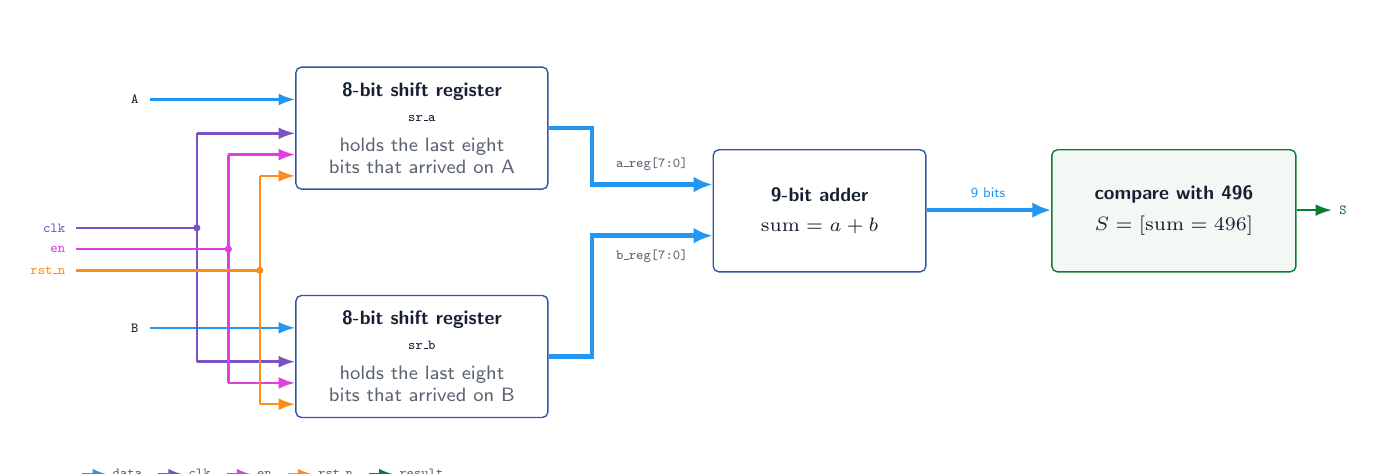
\begin{tikzpicture}[figfont]

\tikzset{
  blk/.style={fbox, minimum width=3.2cm, minimum height=1.55cm, align=center,
    inner sep=5pt},
  jdot/.style={circle, fill=#1, inner sep=0pt, minimum size=2.6pt},
}

% ---- the two registers -------------------------------------------------
\node[blk, anchor=north west] (sra) at (3.4,0)
  {{\bfseries 8-bit shift register}\\[1pt]
   {\ttfamily\tiny sr\_a}\\[3pt]
   \textcolor{figsoft}{holds the last eight}\\
   \textcolor{figsoft}{bits that arrived on A}};

\node[blk, anchor=north west] (srb) at (3.4,-2.9)
  {{\bfseries 8-bit shift register}\\[1pt]
   {\ttfamily\tiny sr\_b}\\[3pt]
   \textcolor{figsoft}{holds the last eight}\\
   \textcolor{figsoft}{bits that arrived on B}};

% ---- serial data in ----------------------------------------------------
\draw[fdata] (1.55,-0.42) -- (3.4,-0.42);
\node[fmono, anchor=east] at (1.45,-0.42) {A};
\draw[fdata] (1.55,-3.32) -- (3.4,-3.32);
\node[fmono, anchor=east] at (1.45,-3.32) {B};

% ---- three separate control rails --------------------------------------
% Each rail enters at its own height, runs to its own vertical, and branches
% to both registers. Filled dots mark real junctions; plain crossings are not
% connections.
\newcommand{\ctrlrail}[6]{% #1 style #2 colour #3 x #4 entry-y #5 up-y #6 down-y
  \draw[#1, -] (0.62,#4) -- (#3,#4);
  \draw[#1, -] (#3,#5) -- (#3,#6);
  \draw[#1] (#3,#5) -- (3.4,#5);
  \draw[#1] (#3,#6) -- (3.4,#6);
  \node[jdot=#2] at (#3,#4) {};
}
\ctrlrail{fclk}{figclkline}{2.15}{-2.05}{-0.85}{-3.75}
\ctrlrail{fen}{figmagenta}{2.55}{-2.32}{-1.12}{-4.02}
\ctrlrail{frst}{figorange}{2.95}{-2.59}{-1.39}{-4.29}

\node[fmono, anchor=east, text=figclkline] at (0.52,-2.05) {clk};
\node[fmono, anchor=east, text=figmagenta] at (0.52,-2.32) {en};
\node[fmono, anchor=east, text=figorange]  at (0.52,-2.59) {rst\_n};

% ---- adder and comparison ----------------------------------------------
\node[blk, anchor=north west, minimum width=2.7cm] (add) at (8.7,-1.05)
  {{\bfseries 9-bit adder}\\[3pt]
   $\mathrm{sum}=a+b$};

\node[blk, anchor=north west, minimum width=3.1cm, draw=figgreen,
      fill=figgreen!5] (cmp) at (13.0,-1.05)
  {{\bfseries compare with 496}\\[3pt]
   $S=[\mathrm{sum}=496]$};

\draw[fbus] (sra.east) -- ++(0.55,0) |- ($(add.north west)+(0,-0.45)$);
\node[fmonosoft, anchor=south] at (7.93,-1.36) {a\_reg[7:0]};
\draw[fbus] (srb.east) -- ++(0.55,0) |- ($(add.north west)+(0,-1.10)$);
\node[fmonosoft, anchor=north] at (7.93,-2.29) {b\_reg[7:0]};

\draw[fbus] ($(add.north east)+(0,-0.775)$) -- ($(cmp.north west)+(0,-0.775)$);
\node[ftag, anchor=south, text=figblue] at (12.2,-1.72) {9 bits};

\draw[fverified] ($(cmp.north east)+(0,-0.775)$) -- ++(0.45,0);
\node[fmono, anchor=west, text=figgreen] at (16.62,-1.83) {S};

% ---- key ---------------------------------------------------------------
\node[ftag, anchor=north west] at (0.62,-5.05)
  {\figkeyitem{fdata}{data}\quad
   \figkeyitem{fclk}{clk}\quad
   \figkeyitem{fen}{en}\quad
   \figkeyitem{frst}{rst\_n}\quad
   \figkeyitem{fverified}{result}};

\end{tikzpicture}
}
  \caption{The warm-up circuit as described.}
  \label{fig:warmup-design}
\end{figure}

\begin{lstlisting}[language=Verilog,caption={The warm-up behavior, abridged from its published source.}]
always @(posedge clk or negedge rst_n)
  if (!rst_n) parallel_out <= 8'b0;
  else if (en) parallel_out <= {parallel_out[6:0], serial_in};

assign sum = a + b;
assign eq  = (val == 9'd496);

comparator496 cmp0 (.val(sum), .eq(S));
\end{lstlisting}

\section{From GDS geometry to wires}

\subsection{What the file describes}

GDS stores polygons tagged with a layer/datatype pair, text labels, reusable cell definitions, and references that place copies of those definitions. This design uses the SkyWater SKY130 process and its high-density standard-cell library. In this process, layers 67--72 are local interconnect (LI1) through metal 5, datatype 20 denotes conductor drawing geometry, datatype 16 denotes pin geometry, and datatype 44 denotes a via cut. Identifying this geometry lets us recover the wires.

\subsection{What the DSU represents logically}

Our extractor gives an integer ID to each conductor polygon. A disjoint-set union (DSU) maintains groups of IDs. At first, every polygon is alone. We do \texttt{union(a,b)} if 1) polygons $a$ and $b$ intersect on the same conducting layer, or 2) a via cut intersects $a$ and $b$. After all unions are completed, $\texttt{find(a)}$ returns the same ID as $\texttt{find(b)}$ iff $a$ and $b$ are connected through such contacts.

We treat each equivalence class as one ideal electrical node, called a net. Note that the DSU records only connectivity; it does not record logical operations, time, direction, or a signal's value.

\vspace{3\baselineskip}
\begin{lstlisting}[language=Python,caption={The 2 physical rules to extract the netlist from GDS, abridged from our extractor.}]
# Same mask layer: exact polygon contact is electrical contact.
for i, polygon in enumerate(layer.polygons):
    for j in layer.tree.query(polygon, predicate="intersects"):
        dsu.union(layer.offset + i, layer.offset + int(j))

# A via cut joins every conductor it touches below to every one above.
for cut in via_cuts:
    for i in conductors_below_touching(cut):
        for j in conductors_above_touching(cut):
            dsu.union(below.offset + i, above.offset + j)
\end{lstlisting}

In the worked example below, the DSU groups 13 conductor drawing polygons on 3 layers through 8 same-layer contacts and 4 via cuts, and attaches 2 cell endpoints. Four overlapping pin shapes bring the extractor's count to 17; they add no new conducting area. The 3 layers are drawn separately in Figure~\ref{fig:warmup-dsu} to make the contacts visible.

\begin{figure}[H]
  \centering
  \includegraphics[width=.95\linewidth]{figures/warmup-net-example.pdf}
  \caption{Recovered warm-up net \texttt{n7}.}
  \label{fig:warmup-dsu}
\end{figure}

\subsection{Attaching names to components}

Standard-cell definitions contain pin labels on LI1. A placed reference carries a transform: a location, a rotation, and possibly a reflection. We apply that transform to the label coordinate and extract which DSU component lies under that point. For example,
\[
  \texttt{sr\_a/\_11\_.X}\longmapsto n7
\]
means that the transformed coordinate of pin label \texttt{X} lies on a conductor polygon whose DSU root was compactly renamed \texttt{n7}. The compact IDs are arbitrary; the endpoint grouping is what matters.

Repeating this for every pin label in the design gives the netlist: a list of placed cells together with the net attached to each of their pins.

\section{From named cells to Boolean equations}

Connectivity tells us which pins share a wire, but cell semantics tell us what those pins compute.

\subsection{Standard cells, masters, and instances}

This design does not lay out transistors gate by gate. It assembles circuits from small, pre-designed components such as AND gates, multiplexers, and flip-flops, each stored once in the GDS as a definition and then placed wherever it is needed. Those definitions have names beginning \texttt{sky130\_fd\_sc\_hd\_\_}.

For example, one embedded definition is named
\[
  \texttt{sky130\_fd\_sc\_hd\_\_mux2\_1}.
\]

The \texttt{mux2} identifies a 2-input multiplexer, and the \texttt{1} identifies its drive-strength variant. Drive strength does not affect the Boolean rule, so we will ignore it. We call a reusable GDS definition a master; an instance is one such placed copy of it. In the warm-up, \texttt{sr\_a/\_11\_} is an instance of the \texttt{mux2\_1} master.

The master defines 4 signal pins:

\begin{center}
  \begin{tabular}{@{}cll@{}}
    \toprule
    Pin & Direction & Meaning \\
    \midrule
    \texttt{A0} & input  & value selected when \texttt{S=0} \\
    \texttt{A1} & input  & value selected when \texttt{S=1} \\
    \texttt{S}  & input  & selection bit \\
    \texttt{X}  & output & selected value \\
    \bottomrule
  \end{tabular}
\end{center}

Consequently, \texttt{sr\_a/\_11\_.X} means ``pin \texttt{X} on this particular placed mux.''

\subsection{Substituting nets into a documented cell rule}

Our geometric reconstruction attaches the 4 pins of this instance to the following nets:

\[
  \begin{array}{c@{\;\longmapsto\;}c}
    \texttt{sr\_a/\_11\_.A0} & n28,\\
    \texttt{sr\_a/\_11\_.A1} & n79,\\
    \texttt{sr\_a/\_11\_.S}  & n80,\\
    \texttt{sr\_a/\_11\_.X}  & n7.
  \end{array}
\]

Each net carries a Boolean value. The 3 input pins read the values on $n28$, $n79$, and $n80$; the output pin drives the result onto $n7$. A mux operates under the following rule:

\[
  X =
  \begin{cases}
    A0,&S=0,\\
    A1,&S=1.
  \end{cases}
  \iff
  n7 =
  \begin{cases}
    n28,&n80=0,\\
    n79,&n80=1.
  \end{cases}
\]

Equivalently,
\[
  n7
  = \operatorname{ite}(n80,n79,n28)
  = (n80\land n79)\lor(\neg n80\land n28),
\]
where $\operatorname{ite}(c,x,y)$ means ``if $c$, then $x$, otherwise $y$.''

In this example, $n80$ is connected to the top-level input \texttt{en}. When \texttt{en=1}, the mux passes $n79$, the output of the preceding shift-register stage, toward the next flip-flop. When \texttt{en=0}, it passes $n28$ back, which is that flip-flop's own output, so the flip-flop retains its current value at the next clock edge.

\subsection{Translating the remaining cells}

We repeat the same substitution for every placed component. For example, a 2-input AND cell obeys

\[
  X=A\land B.
\]

If one particular instance has \texttt{A}$\to n3$,
\texttt{B}$\to n12$, and \texttt{X}$\to n25$, that instance contributes

\[
  n25=n3\land n12.
\]

An inverter contributes a negation. More complicated cells contribute larger
expressions. For example, the documented function of an \texttt{a21o} cell is

\[
  X=(A1\land A2)\lor B1.
\]

This process produces Boolean equations for all combinational cells: components whose outputs depend only on their current inputs. Flip-flops require one additional idea because their outputs depend on an earlier clock edge.

\section{Adding memory and the clock}

A combinational equation relates values at a specific point in time. A flip-flop introduces state. Specifically, an output \texttt{Q} after a rising edge equals \texttt{D} just before that edge. We therefore index state by clock step. If \texttt{n28} is the \texttt{Q} output of \texttt{sr\_a/\_19\_}, then

\[
  n28_{t+1}=\begin{cases}
    0,&\text{if reset is active},\\
    n7_t,&\text{otherwise}.
  \end{cases}
\]

Substituting the mux equation yields

\[
  n28_{t+1}=\operatorname{ite}(\texttt{en}_t,n79_t,n28_t)
  \quad\text{when reset is inactive.}
\]

Figure~\ref{fig:warmup-state} illustrates this rule, both as a circuit and over time.

\begin{figure}[H]
  \centering
  \fitwidth{% One mux, one wire, one flip-flop: where combinational logic stops and state
% begins.
%
% The distinction being taught is about time, which a static schematic cannot
% show, so the schematic is paired with a timing strip over the same three
% nets. The strip is what carries the point: n7 moves whenever its inputs
% move, while n28 moves only at an edge and ignores everything in between.
% The zone tints are fitted to their contents rather than drawn as loose
% rectangles around empty space.
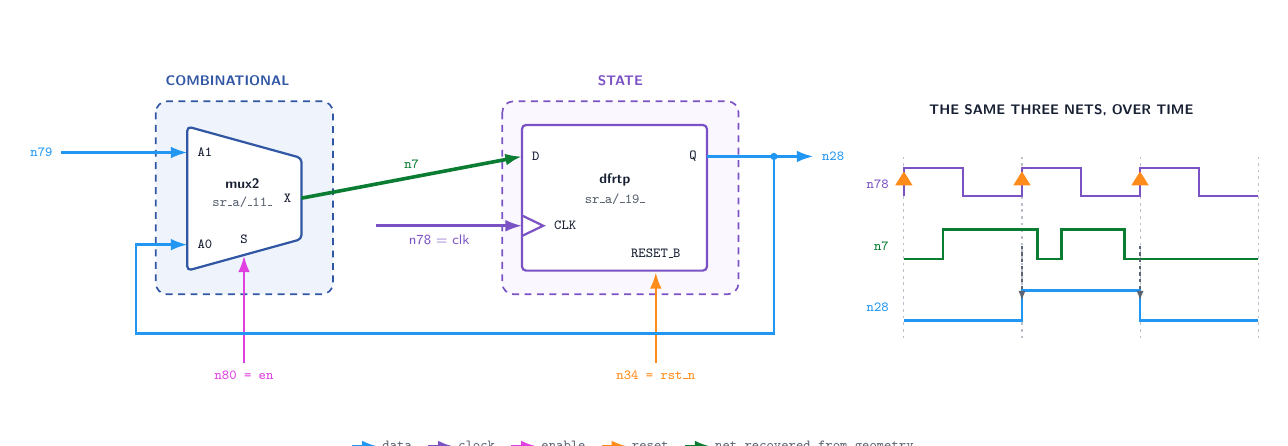
\begin{tikzpicture}[figfont]

\tikzset{
  pinlab/.style={fmono, inner sep=1.5pt},
  zone/.style={rounded corners=4pt, line width=0.6pt,
    dash pattern=on 2.5pt off 2pt},
}

% ======================= the circuit ====================================
\draw[zone, draw=figaccent, fill=figwash] (1.95,-0.30) rectangle (4.20,-2.75);
\node[figfont, anchor=south west, font=\sffamily\tiny\bfseries, text=figaccent]
  at (1.95,-0.22) {COMBINATIONAL};
\draw[zone, draw=figclkline, fill=figviolet!7] (6.35,-0.30) rectangle (9.35,-2.75);
\node[figfont, anchor=south, font=\sffamily\tiny\bfseries, text=figclkline]
  at (7.85,-0.22) {STATE};
% the multiplexer
\filldraw[draw=figaccent, fill=white, line width=0.8pt, rounded corners=1.5pt]
  (2.35,-0.62) -- (3.80,-1.02) -- (3.80,-2.05) -- (2.35,-2.45) -- cycle;
\node[figfont, font=\sffamily\tiny\bfseries] at (3.05,-1.34) {mux2};
\node[fmonosoft] at (3.05,-1.58) {sr\_a/\_11\_};
\node[pinlab, anchor=west] at (2.42,-0.95) {A1};
\node[pinlab, anchor=west] at (2.42,-2.12) {A0};
\node[pinlab, anchor=south] at (3.07,-2.17) {S};
\node[pinlab, anchor=east] at (3.73,-1.53) {X};

\draw[fdata] (0.75,-0.95) -- (2.35,-0.95);
\node[fmono, anchor=east, text=figblue] at (0.68,-0.95) {n79};
\draw[fen] (3.07,-3.62) -- (3.07,-2.26);
\node[fmono, anchor=north, text=figmagenta] at (3.07,-3.68) {n80 = en};

% the net recovered from geometry
\draw[fverified, line width=1.3pt] (3.80,-1.53) -- (6.60,-1.00);
\node[fmono, anchor=south, text=figgreen] at (5.20,-1.20) {n7};

% the flip-flop
\draw[draw=figclkline, fill=white, line width=0.8pt, rounded corners=1.5pt]
  (6.60,-0.60) rectangle (8.95,-2.45);
\node[figfont, font=\sffamily\tiny\bfseries] at (7.78,-1.30) {dfrtp};
\node[fmonosoft] at (7.78,-1.54) {sr\_a/\_19\_};
\node[pinlab, anchor=west] at (6.67,-1.00) {D};
\node[pinlab, anchor=west] at (6.95,-1.88) {CLK};
\node[pinlab, anchor=north] at (8.30,-2.12) {RESET\_B};
\node[pinlab, anchor=east] at (8.88,-1.00) {Q};
\draw[draw=figclkline, line width=0.8pt]
  (6.60,-1.75) -- (6.87,-1.88) -- (6.60,-2.01);

\draw[fclk] (4.75,-1.88) -- (6.60,-1.88);
\node[ftag, anchor=north, text=figclkline] at (5.55,-1.94) {n78 = clk};

\draw[frst] (8.30,-3.62) -- (8.30,-2.47);
\node[fmono, anchor=north, text=figorange] at (8.30,-3.68) {n34 = rst\_n};

\draw[fdata] (8.95,-1.00) -- (10.30,-1.00);
\node[fmono, anchor=west, text=figblue] at (10.37,-1.00) {n28};

% feedback from Q to the mux input
\draw[fdata] (9.80,-1.00) -- (9.80,-3.25) -- (1.70,-3.25) -- (1.70,-2.12)
  -- (2.35,-2.12);
\node[circle, fill=figblue, inner sep=0pt, minimum size=2.6pt] at (9.80,-1.00) {};

% ======================= the same nets, over time =======================
\coordinate (timing-west) at (10.95,-0.22);
\coordinate (timing-east) at (15.95,-0.22);
\node[figfont, anchor=north, font=\sffamily\tiny\bfseries, text=figink]
  at ($(timing-west)!0.5!(timing-east)$) {THE SAME THREE NETS, OVER TIME};

% Stretch the timing strip vertically while preserving its bottom at exactly
% y=-3.31075 cm.  With the lower local bound at -3.05, a vertical scale of
% 0.42 requires shift_y=-3.31075+3.05(0.42)=-2.02975 cm.
\begin{scope}[shift={(11.45,-2.02975)}, x=0.50cm, y=0.42cm]
  \foreach \x in {0,3,6,9}{%
    \draw[figrule, line width=0.4pt, dash pattern=on 1pt off 1.4pt]
      (\x,-3.05) -- (\x,2.45);}

  % the clock, with its rising edges marked on the trace itself
  \node[fmono, anchor=east, text=figclkline] at (-0.3,1.60) {n78};
  \draw[figclkline, line width=0.8pt]
    (0,1.25) -- (0,2.10) -- (1.5,2.10) -- (1.5,1.25) -- (3,1.25) -- (3,2.10) --
    (4.5,2.10) -- (4.5,1.25) -- (6,1.25) -- (6,2.10) -- (7.5,2.10) --
    (7.5,1.25) -- (9,1.25);
  \foreach \x in {0,3,6}{%
    \fill[figorange] (\x-0.22,1.58) -- (\x+0.22,1.58) -- (\x,2.00) -- cycle;}

  % n7 is free to move whenever its inputs move
  \node[fmono, anchor=east, text=figgreen] at (-0.3,-0.25) {n7};
  \draw[figgreen, line width=0.9pt]
    (0,-0.65) -- (1.0,-0.65) -- (1.0,0.25) -- (3.4,0.25) -- (3.4,-0.65) --
    (4.0,-0.65) -- (4.0,0.25) -- (5.6,0.25) -- (5.6,-0.65) -- (9,-0.65);

  % n28 steps only at an edge, to whatever n7 held just before it
  \node[fmono, anchor=east, text=figblue] at (-0.3,-2.10) {n28};
  \draw[figblue, line width=1.0pt]
    (0,-2.50) -- (3,-2.50) -- (3,-1.60) -- (6,-1.60) -- (6,-2.50) -- (9,-2.50);

  \foreach \x in {3,6}{%
    \draw[figsoft, line width=0.5pt, dash pattern=on 1.2pt off 1.2pt,
          -{Latex[length=1.2mm]}] (\x,-0.25) -- (\x,-1.90);}
\end{scope}

% The full composition spans approximately x=0 to x=16.  Center the key on
% that span instead of aligning it with the left-hand circuit.
\coordinate (figure-west) at (0,-4.55);
\coordinate (figure-east) at (16,-4.55);
\node[ftag, anchor=north] at ($(figure-west)!0.5!(figure-east)$)
  {\figkeyitem{fdata}{data}\quad
   \figkeyitem{fclk}{clock}\quad
   \figkeyitem{fen}{enable}\quad
   \figkeyitem{frst}{reset}\quad
   \figkeyitem{fverified}{net recovered from geometry}};

\end{tikzpicture}
}
  \caption{One mux-to-flip-flop path, shown as a circuit and over time.}
  \label{fig:warmup-state}
\end{figure}

The mux output \texttt{n7} changes whenever its inputs change. The flip-flop copies \texttt{n7} into \texttt{n28} only at a rising clock edge, then holds it. Thus the clock marks when the transition equation applies. Pulling reset low overrides the clock and forces \texttt{n28} to 0.

\section{Turning a clocked circuit into one finite formula}

We give the state vector a separate name at each modeled clock edge and connect adjacent states using the next-state function. We call this unrolling the circuit. This leaves one finite combinational formula.

For the warm-up, applying the transition rule 8 times creates states $Q_{0},Q_{1},\ldots,Q_{8}$. Reset fixes $Q_{0}$; the serial input bits at each step are known values; and we evaluate the final expression for \texttt{S}. Because nothing here is unknown, the warm-up is a check rather than a search: $S$ comes out 1 for $250+246$ and 0 for $1+2$, exactly as the published sample tests require.

The warm-up also ships its routed DEF, which states the true connectivity, so we can compare that against our recovered nets. All 84 signal nets and all 291 endpoints agree: no net is missing an endpoint, none has gained one, none is split into two, and no two are merged into one. Since the recovered circuit agrees with both the sample tests and the DEF, we use the same method on the ASIC.

The ASIC uses exactly this construction, with 1 change: the serial inputs are unknown Boolean variables rather than known bits. Let $Q_t$ be the vector of all 92 flip-flop outputs immediately after edge $t$, and let $I_t$ be the bit presented at the next edge. The transition function $T$ evaluates every recovered combinational equation using $Q_t$, $I_t$, and \texttt{enable}$_t$, then collects the resulting flip-flop outputs. Thus

\[
  Q_{t+1}=T\left(Q_{t},I_{t},\texttt{enable}_{t}\right).
\]

In the supplied waveform, \texttt{example\_inputs.vcd}, there are 121 transitions with \texttt{enable=1}, followed by 1 with \texttt{enable=0}. Therefore, there are states $Q_{0}$ through $Q_{122}$, with the goal being $\texttt{success}\left(Q_{122}\right)=1$. Figure~\ref{fig:unrolling} shows the resulting chain.

\begin{figure}[H]
  \centering
  \fitwidth{% One copy of the circuit per modelled clock edge.
%
% The counts are the point of this figure, so they are given their own row
% rather than being buried in the chain: 121 bits go in, 122 edges are
% modelled, and 123 snapshots exist because one of them precedes every edge.
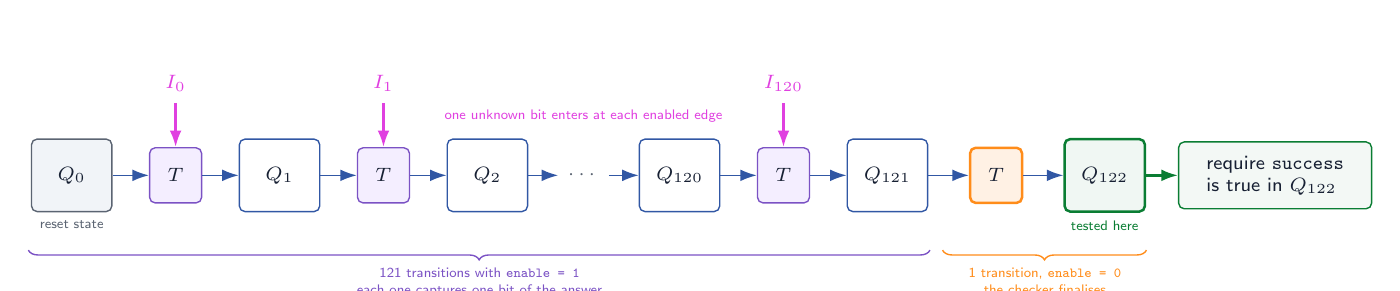
\begin{tikzpicture}[figfont, x=1cm, y=1cm]

\tikzset{
  qstate/.style={fbox, minimum width=1.02cm, minimum height=0.92cm,
    align=center, inner sep=1pt},
  qfirst/.style={qstate, draw=figsoft, fill=figmute},
  qfinal/.style={qstate, draw=figgreen, fill=figgreen!6, line width=0.9pt},
  tstep/.style={fbox, draw=figclkline, fill=figviolet!14,
    minimum width=0.66cm, minimum height=0.7cm, inner sep=1pt},
  tlast/.style={tstep, draw=figorange, fill=figorange!12, line width=0.9pt},
}

% ---- the chain ---------------------------------------------------------
\node[qfirst] (q0)   at (0,0)     {$Q_0$};
\node[tstep]  (t0)   at (1.32,0)  {$T$};
\node[qstate] (q1)   at (2.64,0)  {$Q_1$};
\node[tstep]  (t1)   at (3.96,0)  {$T$};
\node[qstate] (q2)   at (5.28,0)  {$Q_2$};
\node[figsoft] (dots) at (6.5,0)  {$\cdots$};
\node[qstate] (q120) at (7.72,0)  {$Q_{120}$};
\node[tstep]  (t120) at (9.04,0)  {$T$};
\node[qstate] (q121) at (10.36,0) {$Q_{121}$};
\node[tlast]  (t121) at (11.74,0) {$T$};
\node[qfinal] (q122) at (13.12,0) {$Q_{122}$};

\foreach \a/\b in {q0/t0, t0/q1, q1/t1, t1/q2, q2/dots, dots/q120,
                   q120/t120, t120/q121, q121/t121, t121/q122}{%
  \draw[fflow] (\a) -- (\b);}

\node[ftag, anchor=north] at (0,-0.52) {reset state};
\node[ftag, anchor=north, text=figgreen] at (13.12,-0.52) {tested here};

% the bits the solver is free to choose
\foreach \n/\lbl in {t0/{$I_0$}, t1/{$I_1$}, t120/{$I_{120}$}}{%
  \draw[fen] ($(\n.north)+(0,0.56)$) -- (\n.north);
  \node[figfont, text=figmagenta, anchor=south] at ($(\n.north)+(0,0.58)$) {\lbl};}
\node[ftag, text=figmagenta, anchor=south] at (6.5,0.62)
  {one unknown bit enters at each enabled edge};

% ---- what the protocol fixes -------------------------------------------
\draw[decorate, decoration={brace, amplitude=3.5pt, mirror}, draw=figclkline,
      line width=0.5pt] (-0.55,-0.95) -- (10.9,-0.95);
\node[ftag, anchor=north, text=figclkline, align=center] at (5.18,-1.12)
  {121 transitions with {\ttfamily enable = 1}\\each one captures one bit of the answer};

\draw[decorate, decoration={brace, amplitude=3.5pt, mirror}, draw=figorange,
      line width=0.5pt] (11.06,-0.95) -- (13.65,-0.95);
\node[ftag, anchor=north, text=figorange, align=center] at (12.36,-1.12)
  {1 transition, {\ttfamily enable = 0}\\the checker finalises};

\node[fgood, anchor=west, align=left, minimum width=2.45cm, inner sep=5pt]
  (ask) at (14.05,0)
  {require {\ttfamily success}\\is true in $Q_{122}$};
\draw[fverified] (q122) -- (ask);


\end{tikzpicture}
}
  \caption{The puzzle unrolled across 122 clock edges.}
  \label{fig:unrolling}
\end{figure}

The extra disabled transition is necessary because \texttt{success} is stored only after input capture ends.

A Boolean satisfiability (SAT) solver takes a set of constraints over Boolean variables and either returns an assignment that satisfies all of them at once, called a model, or reports \texttt{unsat}, meaning it has proved that no such assignment exists. That is exactly the problem promised in the introduction, so we hand our equations to Z3.

The exported instance contains $11,437$ variables: $121$ unknown inputs and $92\times123=11,316$ state variables. It contains $11,313$ top-level assertions: 88 reset facts, $92\times122$ transition equalities, and 1 final success requirement. The other 4 flip-flops have no reset pin. Under the recovered transition relation, a backward fan-in audit shows that none lies in the transitive fan-in of \texttt{success}, so their unconstrained initial values do not affect the result.

To prove uniqueness, after the first model $b_{0},\ldots,b_{120}$ is found, we add the following clause:

\[
  (I_0\ne b_0)\lor\cdots\lor(I_{120}\ne b_{120}).
\]

It is false for exactly the assignment just found and true for every other 121-bit string, so solving again searches for a different input. Z3 returns \texttt{unsat}, which proves that no other 121-bit input satisfies the recovered circuit.

\section{Result}

The unique 121-bit input is

\begin{center}
  \parbox{.95\linewidth}{\small\bits}
\end{center}

On the next rising edge, \texttt{success} becomes true, and the output circuit emits
\begin{center}
  \Large\texttt{(* TWO STARS *)}
\end{center}

Arranged in the serial stream's row-major order on an $11\times11$ grid, the input has exactly two 1-bits in every row and column, and no two 1-bits touch horizontally, vertically, or diagonally (Figure~\ref{fig:input-grid}). This is oddly reminiscent of Star Battle, leading us to ponder what the mystery regions are.

\begin{figure}[H]
  \centering
  \fitwidth{% Generated by figures/src/make_recovered_board.py - do not edit by hand.
% Source: work/artifacts/logs/06_success_solver_and_uniqueness.txt (chronological bits)
% Regions: work/artifacts/region_map.json (recovered counter schedule)
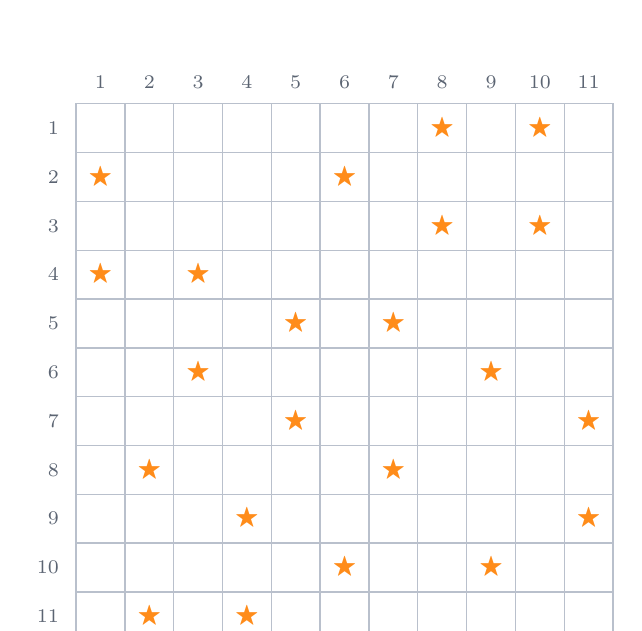
\begin{tikzpicture}[x=0.62cm, y=0.62cm]
  \definecolor{gridink}{HTML}{172033}
  \definecolor{gridsoft}{HTML}{5B6472}
  \definecolor{gridrule}{HTML}{B9C0CC}
  \definecolor{gridstar}{HTML}{FF8C1A}
  \definecolor{gridaccent}{HTML}{3157A4}
  \definecolor{gridok}{HTML}{0A7D33}

  % cells
  \draw[gridrule, line width=0.5pt] (0,10) rectangle (1,11);
  \draw[gridrule, line width=0.5pt] (1,10) rectangle (2,11);
  \draw[gridrule, line width=0.5pt] (2,10) rectangle (3,11);
  \draw[gridrule, line width=0.5pt] (3,10) rectangle (4,11);
  \draw[gridrule, line width=0.5pt] (4,10) rectangle (5,11);
  \draw[gridrule, line width=0.5pt] (5,10) rectangle (6,11);
  \draw[gridrule, line width=0.5pt] (6,10) rectangle (7,11);
  \draw[gridrule, line width=0.5pt] (7,10) rectangle (8,11);
  \draw[gridrule, line width=0.5pt] (8,10) rectangle (9,11);
  \draw[gridrule, line width=0.5pt] (9,10) rectangle (10,11);
  \draw[gridrule, line width=0.5pt] (10,10) rectangle (11,11);
  \draw[gridrule, line width=0.5pt] (0,9) rectangle (1,10);
  \draw[gridrule, line width=0.5pt] (1,9) rectangle (2,10);
  \draw[gridrule, line width=0.5pt] (2,9) rectangle (3,10);
  \draw[gridrule, line width=0.5pt] (3,9) rectangle (4,10);
  \draw[gridrule, line width=0.5pt] (4,9) rectangle (5,10);
  \draw[gridrule, line width=0.5pt] (5,9) rectangle (6,10);
  \draw[gridrule, line width=0.5pt] (6,9) rectangle (7,10);
  \draw[gridrule, line width=0.5pt] (7,9) rectangle (8,10);
  \draw[gridrule, line width=0.5pt] (8,9) rectangle (9,10);
  \draw[gridrule, line width=0.5pt] (9,9) rectangle (10,10);
  \draw[gridrule, line width=0.5pt] (10,9) rectangle (11,10);
  \draw[gridrule, line width=0.5pt] (0,8) rectangle (1,9);
  \draw[gridrule, line width=0.5pt] (1,8) rectangle (2,9);
  \draw[gridrule, line width=0.5pt] (2,8) rectangle (3,9);
  \draw[gridrule, line width=0.5pt] (3,8) rectangle (4,9);
  \draw[gridrule, line width=0.5pt] (4,8) rectangle (5,9);
  \draw[gridrule, line width=0.5pt] (5,8) rectangle (6,9);
  \draw[gridrule, line width=0.5pt] (6,8) rectangle (7,9);
  \draw[gridrule, line width=0.5pt] (7,8) rectangle (8,9);
  \draw[gridrule, line width=0.5pt] (8,8) rectangle (9,9);
  \draw[gridrule, line width=0.5pt] (9,8) rectangle (10,9);
  \draw[gridrule, line width=0.5pt] (10,8) rectangle (11,9);
  \draw[gridrule, line width=0.5pt] (0,7) rectangle (1,8);
  \draw[gridrule, line width=0.5pt] (1,7) rectangle (2,8);
  \draw[gridrule, line width=0.5pt] (2,7) rectangle (3,8);
  \draw[gridrule, line width=0.5pt] (3,7) rectangle (4,8);
  \draw[gridrule, line width=0.5pt] (4,7) rectangle (5,8);
  \draw[gridrule, line width=0.5pt] (5,7) rectangle (6,8);
  \draw[gridrule, line width=0.5pt] (6,7) rectangle (7,8);
  \draw[gridrule, line width=0.5pt] (7,7) rectangle (8,8);
  \draw[gridrule, line width=0.5pt] (8,7) rectangle (9,8);
  \draw[gridrule, line width=0.5pt] (9,7) rectangle (10,8);
  \draw[gridrule, line width=0.5pt] (10,7) rectangle (11,8);
  \draw[gridrule, line width=0.5pt] (0,6) rectangle (1,7);
  \draw[gridrule, line width=0.5pt] (1,6) rectangle (2,7);
  \draw[gridrule, line width=0.5pt] (2,6) rectangle (3,7);
  \draw[gridrule, line width=0.5pt] (3,6) rectangle (4,7);
  \draw[gridrule, line width=0.5pt] (4,6) rectangle (5,7);
  \draw[gridrule, line width=0.5pt] (5,6) rectangle (6,7);
  \draw[gridrule, line width=0.5pt] (6,6) rectangle (7,7);
  \draw[gridrule, line width=0.5pt] (7,6) rectangle (8,7);
  \draw[gridrule, line width=0.5pt] (8,6) rectangle (9,7);
  \draw[gridrule, line width=0.5pt] (9,6) rectangle (10,7);
  \draw[gridrule, line width=0.5pt] (10,6) rectangle (11,7);
  \draw[gridrule, line width=0.5pt] (0,5) rectangle (1,6);
  \draw[gridrule, line width=0.5pt] (1,5) rectangle (2,6);
  \draw[gridrule, line width=0.5pt] (2,5) rectangle (3,6);
  \draw[gridrule, line width=0.5pt] (3,5) rectangle (4,6);
  \draw[gridrule, line width=0.5pt] (4,5) rectangle (5,6);
  \draw[gridrule, line width=0.5pt] (5,5) rectangle (6,6);
  \draw[gridrule, line width=0.5pt] (6,5) rectangle (7,6);
  \draw[gridrule, line width=0.5pt] (7,5) rectangle (8,6);
  \draw[gridrule, line width=0.5pt] (8,5) rectangle (9,6);
  \draw[gridrule, line width=0.5pt] (9,5) rectangle (10,6);
  \draw[gridrule, line width=0.5pt] (10,5) rectangle (11,6);
  \draw[gridrule, line width=0.5pt] (0,4) rectangle (1,5);
  \draw[gridrule, line width=0.5pt] (1,4) rectangle (2,5);
  \draw[gridrule, line width=0.5pt] (2,4) rectangle (3,5);
  \draw[gridrule, line width=0.5pt] (3,4) rectangle (4,5);
  \draw[gridrule, line width=0.5pt] (4,4) rectangle (5,5);
  \draw[gridrule, line width=0.5pt] (5,4) rectangle (6,5);
  \draw[gridrule, line width=0.5pt] (6,4) rectangle (7,5);
  \draw[gridrule, line width=0.5pt] (7,4) rectangle (8,5);
  \draw[gridrule, line width=0.5pt] (8,4) rectangle (9,5);
  \draw[gridrule, line width=0.5pt] (9,4) rectangle (10,5);
  \draw[gridrule, line width=0.5pt] (10,4) rectangle (11,5);
  \draw[gridrule, line width=0.5pt] (0,3) rectangle (1,4);
  \draw[gridrule, line width=0.5pt] (1,3) rectangle (2,4);
  \draw[gridrule, line width=0.5pt] (2,3) rectangle (3,4);
  \draw[gridrule, line width=0.5pt] (3,3) rectangle (4,4);
  \draw[gridrule, line width=0.5pt] (4,3) rectangle (5,4);
  \draw[gridrule, line width=0.5pt] (5,3) rectangle (6,4);
  \draw[gridrule, line width=0.5pt] (6,3) rectangle (7,4);
  \draw[gridrule, line width=0.5pt] (7,3) rectangle (8,4);
  \draw[gridrule, line width=0.5pt] (8,3) rectangle (9,4);
  \draw[gridrule, line width=0.5pt] (9,3) rectangle (10,4);
  \draw[gridrule, line width=0.5pt] (10,3) rectangle (11,4);
  \draw[gridrule, line width=0.5pt] (0,2) rectangle (1,3);
  \draw[gridrule, line width=0.5pt] (1,2) rectangle (2,3);
  \draw[gridrule, line width=0.5pt] (2,2) rectangle (3,3);
  \draw[gridrule, line width=0.5pt] (3,2) rectangle (4,3);
  \draw[gridrule, line width=0.5pt] (4,2) rectangle (5,3);
  \draw[gridrule, line width=0.5pt] (5,2) rectangle (6,3);
  \draw[gridrule, line width=0.5pt] (6,2) rectangle (7,3);
  \draw[gridrule, line width=0.5pt] (7,2) rectangle (8,3);
  \draw[gridrule, line width=0.5pt] (8,2) rectangle (9,3);
  \draw[gridrule, line width=0.5pt] (9,2) rectangle (10,3);
  \draw[gridrule, line width=0.5pt] (10,2) rectangle (11,3);
  \draw[gridrule, line width=0.5pt] (0,1) rectangle (1,2);
  \draw[gridrule, line width=0.5pt] (1,1) rectangle (2,2);
  \draw[gridrule, line width=0.5pt] (2,1) rectangle (3,2);
  \draw[gridrule, line width=0.5pt] (3,1) rectangle (4,2);
  \draw[gridrule, line width=0.5pt] (4,1) rectangle (5,2);
  \draw[gridrule, line width=0.5pt] (5,1) rectangle (6,2);
  \draw[gridrule, line width=0.5pt] (6,1) rectangle (7,2);
  \draw[gridrule, line width=0.5pt] (7,1) rectangle (8,2);
  \draw[gridrule, line width=0.5pt] (8,1) rectangle (9,2);
  \draw[gridrule, line width=0.5pt] (9,1) rectangle (10,2);
  \draw[gridrule, line width=0.5pt] (10,1) rectangle (11,2);
  \draw[gridrule, line width=0.5pt] (0,0) rectangle (1,1);
  \draw[gridrule, line width=0.5pt] (1,0) rectangle (2,1);
  \draw[gridrule, line width=0.5pt] (2,0) rectangle (3,1);
  \draw[gridrule, line width=0.5pt] (3,0) rectangle (4,1);
  \draw[gridrule, line width=0.5pt] (4,0) rectangle (5,1);
  \draw[gridrule, line width=0.5pt] (5,0) rectangle (6,1);
  \draw[gridrule, line width=0.5pt] (6,0) rectangle (7,1);
  \draw[gridrule, line width=0.5pt] (7,0) rectangle (8,1);
  \draw[gridrule, line width=0.5pt] (8,0) rectangle (9,1);
  \draw[gridrule, line width=0.5pt] (9,0) rectangle (10,1);
  \draw[gridrule, line width=0.5pt] (10,0) rectangle (11,1);

  % bold boundaries between circuit-derived regions
  % \draw[gridink, line width=0.9pt] (0,11) -- (1,11);
  % \draw[gridink, line width=0.9pt] (0,10) -- (0,11);
  % \draw[gridink, line width=0.9pt] (1,11) -- (2,11);
  % \draw[gridink, line width=0.9pt] (2,11) -- (3,11);
  % \draw[gridink, line width=0.9pt] (3,11) -- (4,11);
  % \draw[gridink, line width=0.9pt] (4,11) -- (5,11);
  % \draw[gridink, line width=0.9pt] (5,11) -- (6,11);
  % \draw[gridink, line width=0.9pt] (5,10) -- (5,11);
  % \draw[gridink, line width=0.9pt] (6,11) -- (7,11);
  % \draw[gridink, line width=0.9pt] (7,11) -- (8,11);
  % \draw[gridink, line width=0.9pt] (7,10) -- (7,11);
  % \draw[gridink, line width=0.9pt] (8,11) -- (9,11);
  % \draw[gridink, line width=0.9pt] (8,10) -- (8,11);
  % \draw[gridink, line width=0.9pt] (9,11) -- (10,11);
  % \draw[gridink, line width=0.9pt] (10,11) -- (11,11);
  % \draw[gridink, line width=0.9pt] (10,10) -- (10,11);
  % \draw[gridink, line width=0.9pt] (11,10) -- (11,11);
  % \draw[gridink, line width=0.9pt] (0,9) -- (0,10);
  % \draw[gridink, line width=0.9pt] (2,10) -- (3,10);
  % \draw[gridink, line width=0.9pt] (2,9) -- (2,10);
  % \draw[gridink, line width=0.9pt] (3,9) -- (3,10);
  % \draw[gridink, line width=0.9pt] (5,9) -- (5,10);
  % \draw[gridink, line width=0.9pt] (6,10) -- (7,10);
  % \draw[gridink, line width=0.9pt] (6,9) -- (6,10);
  % \draw[gridink, line width=0.9pt] (8,9) -- (8,10);
  % \draw[gridink, line width=0.9pt] (10,9) -- (10,10);
  % \draw[gridink, line width=0.9pt] (11,9) -- (11,10);
  % \draw[gridink, line width=0.9pt] (0,8) -- (0,9);
  % \draw[gridink, line width=0.9pt] (2,8) -- (2,9);
  % \draw[gridink, line width=0.9pt] (3,9) -- (4,9);
  % \draw[gridink, line width=0.9pt] (3,8) -- (3,9);
  % \draw[gridink, line width=0.9pt] (4,9) -- (5,9);
  % \draw[gridink, line width=0.9pt] (6,9) -- (7,9);
  % \draw[gridink, line width=0.9pt] (7,8) -- (7,9);
  % \draw[gridink, line width=0.9pt] (8,9) -- (9,9);
  % \draw[gridink, line width=0.9pt] (9,8) -- (9,9);
  % \draw[gridink, line width=0.9pt] (10,8) -- (10,9);
  % \draw[gridink, line width=0.9pt] (11,8) -- (11,9);
  % \draw[gridink, line width=0.9pt] (0,7) -- (0,8);
  % \draw[gridink, line width=0.9pt] (2,7) -- (2,8);
  % \draw[gridink, line width=0.9pt] (3,7) -- (3,8);
  % \draw[gridink, line width=0.9pt] (4,8) -- (5,8);
  % \draw[gridink, line width=0.9pt] (4,7) -- (4,8);
  % \draw[gridink, line width=0.9pt] (5,8) -- (6,8);
  % \draw[gridink, line width=0.9pt] (6,8) -- (7,8);
  % \draw[gridink, line width=0.9pt] (7,8) -- (8,8);
  % \draw[gridink, line width=0.9pt] (7,7) -- (7,8);
  % \draw[gridink, line width=0.9pt] (8,7) -- (8,8);
  % \draw[gridink, line width=0.9pt] (9,8) -- (10,8);
  % \draw[gridink, line width=0.9pt] (10,7) -- (10,8);
  % \draw[gridink, line width=0.9pt] (11,7) -- (11,8);
  % \draw[gridink, line width=0.9pt] (0,7) -- (1,7);
  % \draw[gridink, line width=0.9pt] (0,6) -- (0,7);
  % \draw[gridink, line width=0.9pt] (1,6) -- (1,7);
  % \draw[gridink, line width=0.9pt] (2,6) -- (2,7);
  % \draw[gridink, line width=0.9pt] (3,6) -- (3,7);
  % \draw[gridink, line width=0.9pt] (4,6) -- (4,7);
  % \draw[gridink, line width=0.9pt] (5,7) -- (6,7);
  % \draw[gridink, line width=0.9pt] (5,6) -- (5,7);
  % \draw[gridink, line width=0.9pt] (6,7) -- (7,7);
  % \draw[gridink, line width=0.9pt] (8,7) -- (9,7);
  % \draw[gridink, line width=0.9pt] (9,7) -- (10,7);
  % \draw[gridink, line width=0.9pt] (11,6) -- (11,7);
  % \draw[gridink, line width=0.9pt] (0,5) -- (0,6);
  % \draw[gridink, line width=0.9pt] (1,6) -- (2,6);
  % \draw[gridink, line width=0.9pt] (3,5) -- (3,6);
  % \draw[gridink, line width=0.9pt] (4,5) -- (4,6);
  % \draw[gridink, line width=0.9pt] (5,6) -- (6,6);
  % \draw[gridink, line width=0.9pt] (6,6) -- (7,6);
  % \draw[gridink, line width=0.9pt] (7,5) -- (7,6);
  % \draw[gridink, line width=0.9pt] (8,6) -- (9,6);
  % \draw[gridink, line width=0.9pt] (8,5) -- (8,6);
  % \draw[gridink, line width=0.9pt] (9,6) -- (10,6);
  % \draw[gridink, line width=0.9pt] (10,6) -- (11,6);
  % \draw[gridink, line width=0.9pt] (11,5) -- (11,6);
  % \draw[gridink, line width=0.9pt] (0,5) -- (1,5);
  % \draw[gridink, line width=0.9pt] (0,4) -- (0,5);
  % \draw[gridink, line width=0.9pt] (1,5) -- (2,5);
  % \draw[gridink, line width=0.9pt] (2,5) -- (3,5);
  % \draw[gridink, line width=0.9pt] (4,5) -- (5,5);
  % \draw[gridink, line width=0.9pt] (5,5) -- (6,5);
  % \draw[gridink, line width=0.9pt] (6,4) -- (6,5);
  % \draw[gridink, line width=0.9pt] (7,4) -- (7,5);
  % \draw[gridink, line width=0.9pt] (8,4) -- (8,5);
  % \draw[gridink, line width=0.9pt] (9,5) -- (10,5);
  % \draw[gridink, line width=0.9pt] (9,4) -- (9,5);
  % \draw[gridink, line width=0.9pt] (10,5) -- (11,5);
  % \draw[gridink, line width=0.9pt] (11,4) -- (11,5);
  % \draw[gridink, line width=0.9pt] (0,3) -- (0,4);
  % \draw[gridink, line width=0.9pt] (1,4) -- (2,4);
  % \draw[gridink, line width=0.9pt] (1,3) -- (1,4);
  % \draw[gridink, line width=0.9pt] (2,4) -- (3,4);
  % \draw[gridink, line width=0.9pt] (3,4) -- (4,4);
  % \draw[gridink, line width=0.9pt] (4,4) -- (5,4);
  % \draw[gridink, line width=0.9pt] (4,3) -- (4,4);
  % \draw[gridink, line width=0.9pt] (5,4) -- (6,4);
  % \draw[gridink, line width=0.9pt] (7,3) -- (7,4);
  % \draw[gridink, line width=0.9pt] (8,3) -- (8,4);
  % \draw[gridink, line width=0.9pt] (9,3) -- (9,4);
  % \draw[gridink, line width=0.9pt] (11,3) -- (11,4);
  % \draw[gridink, line width=0.9pt] (0,2) -- (0,3);
  % \draw[gridink, line width=0.9pt] (1,2) -- (1,3);
  % \draw[gridink, line width=0.9pt] (3,3) -- (4,3);
  % \draw[gridink, line width=0.9pt] (3,2) -- (3,3);
  % \draw[gridink, line width=0.9pt] (4,3) -- (5,3);
  % \draw[gridink, line width=0.9pt] (4,2) -- (4,3);
  % \draw[gridink, line width=0.9pt] (5,3) -- (6,3);
  % \draw[gridink, line width=0.9pt] (6,3) -- (7,3);
  % \draw[gridink, line width=0.9pt] (8,2) -- (8,3);
  % \draw[gridink, line width=0.9pt] (9,2) -- (9,3);
  % \draw[gridink, line width=0.9pt] (11,2) -- (11,3);
  % \draw[gridink, line width=0.9pt] (0,1) -- (0,2);
  % \draw[gridink, line width=0.9pt] (1,2) -- (2,2);
  % \draw[gridink, line width=0.9pt] (2,1) -- (2,2);
  % \draw[gridink, line width=0.9pt] (3,1) -- (3,2);
  % \draw[gridink, line width=0.9pt] (4,2) -- (5,2);
  % \draw[gridink, line width=0.9pt] (5,1) -- (5,2);
  % \draw[gridink, line width=0.9pt] (8,1) -- (8,2);
  % \draw[gridink, line width=0.9pt] (9,2) -- (10,2);
  % \draw[gridink, line width=0.9pt] (10,2) -- (11,2);
  % \draw[gridink, line width=0.9pt] (11,1) -- (11,2);
  % \draw[gridink, line width=0.9pt] (0,0) -- (0,1);
  % \draw[gridink, line width=0.9pt] (0,0) -- (1,0);
  % \draw[gridink, line width=0.9pt] (1,1) -- (2,1);
  % \draw[gridink, line width=0.9pt] (1,0) -- (1,1);
  % \draw[gridink, line width=0.9pt] (1,0) -- (2,0);
  % \draw[gridink, line width=0.9pt] (2,0) -- (3,0);
  % \draw[gridink, line width=0.9pt] (3,0) -- (3,1);
  % \draw[gridink, line width=0.9pt] (3,0) -- (4,0);
  % \draw[gridink, line width=0.9pt] (4,1) -- (5,1);
  % \draw[gridink, line width=0.9pt] (4,0) -- (4,1);
  % \draw[gridink, line width=0.9pt] (4,0) -- (5,0);
  % \draw[gridink, line width=0.9pt] (5,0) -- (6,0);
  % \draw[gridink, line width=0.9pt] (6,0) -- (7,0);
  % \draw[gridink, line width=0.9pt] (7,0) -- (8,0);
  % \draw[gridink, line width=0.9pt] (8,1) -- (9,1);
  % \draw[gridink, line width=0.9pt] (8,0) -- (9,0);
  % \draw[gridink, line width=0.9pt] (9,1) -- (10,1);
  % \draw[gridink, line width=0.9pt] (9,0) -- (10,0);
  % \draw[gridink, line width=0.9pt] (10,1) -- (11,1);
  % \draw[gridink, line width=0.9pt] (10,0) -- (11,0);
  % \draw[gridink, line width=0.9pt] (11,0) -- (11,1);

  % heavier outlines for the three recovered JSC glyph regions
  % \draw[gridink, line width=2pt] (2,10) -- (3,10);
  % \draw[gridink, line width=2pt] (2,9) -- (2,10);
  % \draw[gridink, line width=2pt] (3,9) -- (3,10);
  % \draw[gridink, line width=2pt] (2,8) -- (2,9);
  % \draw[gridink, line width=2pt] (3,8) -- (3,9);
  % \draw[gridink, line width=2pt] (2,7) -- (2,8);
  % \draw[gridink, line width=2pt] (3,7) -- (3,8);
  % \draw[gridink, line width=2pt] (4,8) -- (5,8);
  % \draw[gridink, line width=2pt] (4,7) -- (4,8);
  % \draw[gridink, line width=2pt] (5,8) -- (6,8);
  % \draw[gridink, line width=2pt] (5,7) -- (6,7);
  % \draw[gridink, line width=2pt] (6,8) -- (7,8);
  % \draw[gridink, line width=2pt] (6,7) -- (7,7);
  % \draw[gridink, line width=2pt] (7,7) -- (7,8);
  % \draw[gridink, line width=2pt] (0,7) -- (1,7);
  % \draw[gridink, line width=2pt] (0,6) -- (0,7);
  % \draw[gridink, line width=2pt] (1,6) -- (1,7);
  % \draw[gridink, line width=2pt] (2,6) -- (2,7);
  % \draw[gridink, line width=2pt] (3,6) -- (3,7);
  % \draw[gridink, line width=2pt] (4,6) -- (4,7);
  % \draw[gridink, line width=2pt] (5,6) -- (5,7);
  % \draw[gridink, line width=2pt] (0,5) -- (0,6);
  % \draw[gridink, line width=2pt] (0,5) -- (1,5);
  % \draw[gridink, line width=2pt] (1,6) -- (2,6);
  % \draw[gridink, line width=2pt] (1,5) -- (2,5);
  % \draw[gridink, line width=2pt] (2,5) -- (3,5);
  % \draw[gridink, line width=2pt] (3,5) -- (3,6);
  % \draw[gridink, line width=2pt] (4,5) -- (4,6);
  % \draw[gridink, line width=2pt] (4,5) -- (5,5);
  % \draw[gridink, line width=2pt] (5,6) -- (6,6);
  % \draw[gridink, line width=2pt] (5,5) -- (6,5);
  % \draw[gridink, line width=2pt] (6,6) -- (7,6);
  % \draw[gridink, line width=2pt] (7,5) -- (7,6);
  % \draw[gridink, line width=2pt] (8,6) -- (9,6);
  % \draw[gridink, line width=2pt] (8,5) -- (8,6);
  % \draw[gridink, line width=2pt] (9,6) -- (10,6);
  % \draw[gridink, line width=2pt] (9,5) -- (10,5);
  % \draw[gridink, line width=2pt] (10,6) -- (11,6);
  % \draw[gridink, line width=2pt] (10,5) -- (11,5);
  % \draw[gridink, line width=2pt] (11,5) -- (11,6);
  % \draw[gridink, line width=2pt] (6,4) -- (6,5);
  % \draw[gridink, line width=2pt] (7,4) -- (7,5);
  % \draw[gridink, line width=2pt] (8,4) -- (8,5);
  % \draw[gridink, line width=2pt] (9,4) -- (9,5);
  % \draw[gridink, line width=2pt] (4,4) -- (5,4);
  % \draw[gridink, line width=2pt] (4,3) -- (4,4);
  % \draw[gridink, line width=2pt] (4,3) -- (5,3);
  % \draw[gridink, line width=2pt] (5,4) -- (6,4);
  % \draw[gridink, line width=2pt] (5,3) -- (6,3);
  % \draw[gridink, line width=2pt] (6,3) -- (7,3);
  % \draw[gridink, line width=2pt] (7,3) -- (7,4);
  % \draw[gridink, line width=2pt] (8,3) -- (8,4);
  % \draw[gridink, line width=2pt] (9,3) -- (9,4);
  % \draw[gridink, line width=2pt] (8,2) -- (8,3);
  % \draw[gridink, line width=2pt] (9,2) -- (9,3);
  % \draw[gridink, line width=2pt] (8,1) -- (8,2);
  % \draw[gridink, line width=2pt] (8,1) -- (9,1);
  % \draw[gridink, line width=2pt] (9,2) -- (10,2);
  % \draw[gridink, line width=2pt] (9,1) -- (10,1);
  % \draw[gridink, line width=2pt] (10,2) -- (11,2);
  % \draw[gridink, line width=2pt] (10,1) -- (11,1);
  % \draw[gridink, line width=2pt] (11,1) -- (11,2);

  % stars: one per 1 bit
  \node[gridstar] at (7.5,10.5) {\small$\bigstar$};
  \node[gridstar] at (9.5,10.5) {\small$\bigstar$};
  \node[gridstar] at (0.5,9.5) {\small$\bigstar$};
  \node[gridstar] at (5.5,9.5) {\small$\bigstar$};
  \node[gridstar] at (7.5,8.5) {\small$\bigstar$};
  \node[gridstar] at (9.5,8.5) {\small$\bigstar$};
  \node[gridstar] at (0.5,7.5) {\small$\bigstar$};
  \node[gridstar] at (2.5,7.5) {\small$\bigstar$};
  \node[gridstar] at (4.5,6.5) {\small$\bigstar$};
  \node[gridstar] at (6.5,6.5) {\small$\bigstar$};
  \node[gridstar] at (2.5,5.5) {\small$\bigstar$};
  \node[gridstar] at (8.5,5.5) {\small$\bigstar$};
  \node[gridstar] at (4.5,4.5) {\small$\bigstar$};
  \node[gridstar] at (10.5,4.5) {\small$\bigstar$};
  \node[gridstar] at (1.5,3.5) {\small$\bigstar$};
  \node[gridstar] at (6.5,3.5) {\small$\bigstar$};
  \node[gridstar] at (3.5,2.5) {\small$\bigstar$};
  \node[gridstar] at (10.5,2.5) {\small$\bigstar$};
  \node[gridstar] at (5.5,1.5) {\small$\bigstar$};
  \node[gridstar] at (8.5,1.5) {\small$\bigstar$};
  \node[gridstar] at (1.5,0.5) {\small$\bigstar$};
  \node[gridstar] at (3.5,0.5) {\small$\bigstar$};

  % row and column indices, and the per-line star counts
  \node[gridsoft, anchor=east, font=\scriptsize] at (-0.15,10.5) {1};
  % \node[gridok, anchor=west, font=\scriptsize] at (11.2,10.5) {2};
  \node[gridsoft, anchor=east, font=\scriptsize] at (-0.15,9.5) {2};
  % \node[gridok, anchor=west, font=\scriptsize] at (11.2,9.5) {2};
  \node[gridsoft, anchor=east, font=\scriptsize] at (-0.15,8.5) {3};
  % \node[gridok, anchor=west, font=\scriptsize] at (11.2,8.5) {2};
  \node[gridsoft, anchor=east, font=\scriptsize] at (-0.15,7.5) {4};
  % \node[gridok, anchor=west, font=\scriptsize] at (11.2,7.5) {2};
  \node[gridsoft, anchor=east, font=\scriptsize] at (-0.15,6.5) {5};
  % \node[gridok, anchor=west, font=\scriptsize] at (11.2,6.5) {2};
  \node[gridsoft, anchor=east, font=\scriptsize] at (-0.15,5.5) {6};
  % \node[gridok, anchor=west, font=\scriptsize] at (11.2,5.5) {2};
  \node[gridsoft, anchor=east, font=\scriptsize] at (-0.15,4.5) {7};
  % \node[gridok, anchor=west, font=\scriptsize] at (11.2,4.5) {2};
  \node[gridsoft, anchor=east, font=\scriptsize] at (-0.15,3.5) {8};
  % \node[gridok, anchor=west, font=\scriptsize] at (11.2,3.5) {2};
  \node[gridsoft, anchor=east, font=\scriptsize] at (-0.15,2.5) {9};
  % \node[gridok, anchor=west, font=\scriptsize] at (11.2,2.5) {2};
  \node[gridsoft, anchor=east, font=\scriptsize] at (-0.15,1.5) {10};
  % \node[gridok, anchor=west, font=\scriptsize] at (11.2,1.5) {2};
  \node[gridsoft, anchor=east, font=\scriptsize] at (-0.15,0.5) {11};
  % \node[gridok, anchor=west, font=\scriptsize] at (11.2,0.5) {2};
  \node[gridsoft, anchor=south, font=\scriptsize] at (0.5,11.12) {1};
  % \node[gridok, anchor=north, font=\scriptsize] at (0.5,-0.16) {2};
  \node[gridsoft, anchor=south, font=\scriptsize] at (1.5,11.12) {2};
  % \node[gridok, anchor=north, font=\scriptsize] at (1.5,-0.16) {2};
  \node[gridsoft, anchor=south, font=\scriptsize] at (2.5,11.12) {3};
  % \node[gridok, anchor=north, font=\scriptsize] at (2.5,-0.16) {2};
  \node[gridsoft, anchor=south, font=\scriptsize] at (3.5,11.12) {4};
  % \node[gridok, anchor=north, font=\scriptsize] at (3.5,-0.16) {2};
  \node[gridsoft, anchor=south, font=\scriptsize] at (4.5,11.12) {5};
  % \node[gridok, anchor=north, font=\scriptsize] at (4.5,-0.16) {2};
  \node[gridsoft, anchor=south, font=\scriptsize] at (5.5,11.12) {6};
  % \node[gridok, anchor=north, font=\scriptsize] at (5.5,-0.16) {2};
  \node[gridsoft, anchor=south, font=\scriptsize] at (6.5,11.12) {7};
  % \node[gridok, anchor=north, font=\scriptsize] at (6.5,-0.16) {2};
  \node[gridsoft, anchor=south, font=\scriptsize] at (7.5,11.12) {8};
  % \node[gridok, anchor=north, font=\scriptsize] at (7.5,-0.16) {2};
  \node[gridsoft, anchor=south, font=\scriptsize] at (8.5,11.12) {9};
  % \node[gridok, anchor=north, font=\scriptsize] at (8.5,-0.16) {2};
  \node[gridsoft, anchor=south, font=\scriptsize] at (9.5,11.12) {10};
  % \node[gridok, anchor=north, font=\scriptsize] at (9.5,-0.16) {2};
  \node[gridsoft, anchor=south, font=\scriptsize] at (10.5,11.12) {11};
  % \node[gridok, anchor=north, font=\scriptsize] at (10.5,-0.16) {2};
  % \node[gridok, anchor=west, font=\scriptsize] at (11.2,11.12) {per row};
  % \node[gridok, anchor=north east, font=\scriptsize] at (-0.3,-0.16) {per column};

  % % how a bit index becomes a square
  % \draw[gridaccent, line width=0.5pt, -{Latex[length=1.4mm]}] (0.1,12.0) -- (10.9,12.0);
  % \node[gridaccent, anchor=south, font=\scriptsize] at (5.5,12.1) {bits 1--11 arrive first, left to right};
\end{tikzpicture}
}
  \caption{The recovered input in an $11\times11$ grid.}
  \label{fig:input-grid}
\end{figure}

\subsection{Recovering the regions}

Closer inspection of the 92 flip-flops reveals that 44 lie in 2 regular banks of 22. Tracing their next-state equations pairs each bank into eleven 2-bit counters. One bank is selected by column; the other is selected by an irregular position-dependent signal. Because the 121 bits arrive serially in row-major order, the same 11-column selection schedule is reused for every row.

For a concrete example, one pair has low bit \texttt{n717} and high bit \texttt{n509}. Simplifying the gates that drive their D pins gives the following behavior, with $x$ meaning the current input is 1, capture is enabled, and this particular counter is selected:

\begin{center}
  \small
  \begin{tabular}{@{}cccl@{}}
    \toprule
    $x$ & old HL & new HL & meaning \\
    \midrule
    0 & any & unchanged & this cell does not add to the counter \\
    1 & 00 & 01 & first selected star \\
    1 & 01 & 10 & second selected star \\
    1 & 10 or 11 & 11 & third or later star, saturated at 3 \\
    \bottomrule
  \end{tabular}
\end{center}

Thus the remaining problem is to learn which counter is selected at each of the 121 positions. We reset the circuit and feed 0 for every position before $t$. The position machinery still advances, so the selection signals are correct for position $t$, but no star has been counted anywhere and every counter therefore sits at 00. From 00, a selected counter must move to 01 when it sees a star, while an unselected one cannot move at all. So we copy that pre-edge state and evaluate the next state twice, once with $I_t=0$ and once with $I_t=1$. For these 2 counter banks, exactly 1 low flip-flop per bank differs between the 2 evaluations, and it is the low bit of the counter selected at position $t$.

For cell $(1,1)$, the differing low bits are \texttt{n313} in one bank and \texttt{n717} in the other. The \texttt{n313} choice recurs at cells $(2,1),(3,1),\ldots$, identifying column 1. At $(1,2)$ the column bit changes to \texttt{n304}, while the region bit is still \texttt{n717}, so $(1,1)$ and $(1,2)$ must share the same region. At $(1,6)$ the pair is \texttt{n671} and \texttt{n495}: column 6 and a new region. Repeating this comparison for all 121 stream positions yields the complete partition.

The extracted schedule must pass 4 checks: 11 column selectors repeat every row; 11 region selectors cover all 121 cells exactly once; each resulting region is orthogonally connected; and the winning replay leaves every column and region counter at binary 10. All 4 hold, and the resulting reconstruction is Figure~\ref{fig:board}.

\begin{figure}[H]
  \centering
  \fitwidth{% Recovered board with circuit-derived region boundaries.
% Source: work/artifacts/logs/06_success_solver_and_uniqueness.txt (chronological bits)
% Regions: work/artifacts/region_map.json (recovered counter schedule)
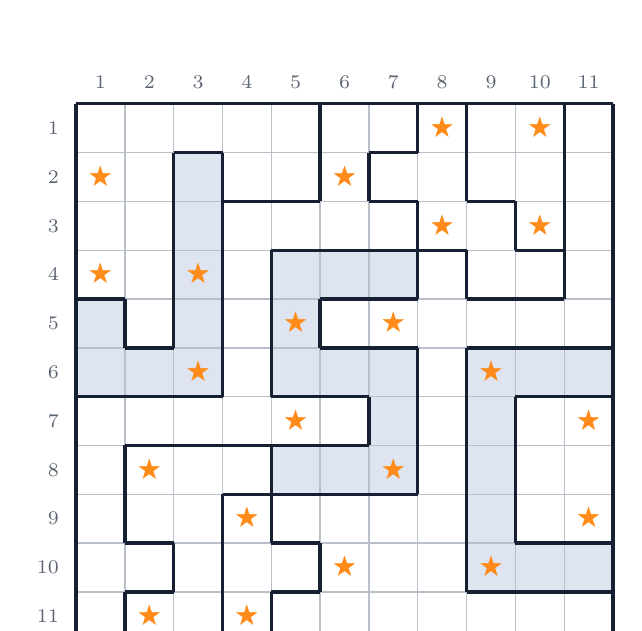
\begin{tikzpicture}[x=0.62cm, y=0.62cm]
  \definecolor{gridink}{HTML}{172033}
  \definecolor{gridsoft}{HTML}{5B6472}
  \definecolor{gridrule}{HTML}{B9C0CC}
  \definecolor{gridstar}{HTML}{FF8C1A}
  \definecolor{gridaccent}{HTML}{3157A4}
  \definecolor{gridok}{HTML}{0A7D33}

  % translucent emphasis for the recovered J, S, and C regions
  \begin{scope}[overlay]
  \fill[gridaccent, opacity=0.16] (2,10) -- (3,10) -- (3,5) -- (0,5)
    -- (0,7) -- (1,7) -- (1,6) -- (2,6) -- cycle;
  \fill[gridaccent, opacity=0.16] (4,8) -- (7,8) -- (7,7) -- (5,7)
    -- (5,6) -- (7,6) -- (7,3) -- (4,3) -- (4,4) -- (6,4)
    -- (6,5) -- (4,5) -- cycle;
  \fill[gridaccent, opacity=0.16] (8,6) -- (11,6) -- (11,5) -- (9,5)
    -- (9,2) -- (11,2) -- (11,1) -- (8,1) -- cycle;
  \end{scope}

  % cells
  \draw[gridrule, line width=0.5pt] (0,10) rectangle (1,11);
  \draw[gridrule, line width=0.5pt] (1,10) rectangle (2,11);
  \draw[gridrule, line width=0.5pt] (2,10) rectangle (3,11);
  \draw[gridrule, line width=0.5pt] (3,10) rectangle (4,11);
  \draw[gridrule, line width=0.5pt] (4,10) rectangle (5,11);
  \draw[gridrule, line width=0.5pt] (5,10) rectangle (6,11);
  \draw[gridrule, line width=0.5pt] (6,10) rectangle (7,11);
  \draw[gridrule, line width=0.5pt] (7,10) rectangle (8,11);
  \draw[gridrule, line width=0.5pt] (8,10) rectangle (9,11);
  \draw[gridrule, line width=0.5pt] (9,10) rectangle (10,11);
  \draw[gridrule, line width=0.5pt] (10,10) rectangle (11,11);
  \draw[gridrule, line width=0.5pt] (0,9) rectangle (1,10);
  \draw[gridrule, line width=0.5pt] (1,9) rectangle (2,10);
  \draw[gridrule, line width=0.5pt] (2,9) rectangle (3,10);
  \draw[gridrule, line width=0.5pt] (3,9) rectangle (4,10);
  \draw[gridrule, line width=0.5pt] (4,9) rectangle (5,10);
  \draw[gridrule, line width=0.5pt] (5,9) rectangle (6,10);
  \draw[gridrule, line width=0.5pt] (6,9) rectangle (7,10);
  \draw[gridrule, line width=0.5pt] (7,9) rectangle (8,10);
  \draw[gridrule, line width=0.5pt] (8,9) rectangle (9,10);
  \draw[gridrule, line width=0.5pt] (9,9) rectangle (10,10);
  \draw[gridrule, line width=0.5pt] (10,9) rectangle (11,10);
  \draw[gridrule, line width=0.5pt] (0,8) rectangle (1,9);
  \draw[gridrule, line width=0.5pt] (1,8) rectangle (2,9);
  \draw[gridrule, line width=0.5pt] (2,8) rectangle (3,9);
  \draw[gridrule, line width=0.5pt] (3,8) rectangle (4,9);
  \draw[gridrule, line width=0.5pt] (4,8) rectangle (5,9);
  \draw[gridrule, line width=0.5pt] (5,8) rectangle (6,9);
  \draw[gridrule, line width=0.5pt] (6,8) rectangle (7,9);
  \draw[gridrule, line width=0.5pt] (7,8) rectangle (8,9);
  \draw[gridrule, line width=0.5pt] (8,8) rectangle (9,9);
  \draw[gridrule, line width=0.5pt] (9,8) rectangle (10,9);
  \draw[gridrule, line width=0.5pt] (10,8) rectangle (11,9);
  \draw[gridrule, line width=0.5pt] (0,7) rectangle (1,8);
  \draw[gridrule, line width=0.5pt] (1,7) rectangle (2,8);
  \draw[gridrule, line width=0.5pt] (2,7) rectangle (3,8);
  \draw[gridrule, line width=0.5pt] (3,7) rectangle (4,8);
  \draw[gridrule, line width=0.5pt] (4,7) rectangle (5,8);
  \draw[gridrule, line width=0.5pt] (5,7) rectangle (6,8);
  \draw[gridrule, line width=0.5pt] (6,7) rectangle (7,8);
  \draw[gridrule, line width=0.5pt] (7,7) rectangle (8,8);
  \draw[gridrule, line width=0.5pt] (8,7) rectangle (9,8);
  \draw[gridrule, line width=0.5pt] (9,7) rectangle (10,8);
  \draw[gridrule, line width=0.5pt] (10,7) rectangle (11,8);
  \draw[gridrule, line width=0.5pt] (0,6) rectangle (1,7);
  \draw[gridrule, line width=0.5pt] (1,6) rectangle (2,7);
  \draw[gridrule, line width=0.5pt] (2,6) rectangle (3,7);
  \draw[gridrule, line width=0.5pt] (3,6) rectangle (4,7);
  \draw[gridrule, line width=0.5pt] (4,6) rectangle (5,7);
  \draw[gridrule, line width=0.5pt] (5,6) rectangle (6,7);
  \draw[gridrule, line width=0.5pt] (6,6) rectangle (7,7);
  \draw[gridrule, line width=0.5pt] (7,6) rectangle (8,7);
  \draw[gridrule, line width=0.5pt] (8,6) rectangle (9,7);
  \draw[gridrule, line width=0.5pt] (9,6) rectangle (10,7);
  \draw[gridrule, line width=0.5pt] (10,6) rectangle (11,7);
  \draw[gridrule, line width=0.5pt] (0,5) rectangle (1,6);
  \draw[gridrule, line width=0.5pt] (1,5) rectangle (2,6);
  \draw[gridrule, line width=0.5pt] (2,5) rectangle (3,6);
  \draw[gridrule, line width=0.5pt] (3,5) rectangle (4,6);
  \draw[gridrule, line width=0.5pt] (4,5) rectangle (5,6);
  \draw[gridrule, line width=0.5pt] (5,5) rectangle (6,6);
  \draw[gridrule, line width=0.5pt] (6,5) rectangle (7,6);
  \draw[gridrule, line width=0.5pt] (7,5) rectangle (8,6);
  \draw[gridrule, line width=0.5pt] (8,5) rectangle (9,6);
  \draw[gridrule, line width=0.5pt] (9,5) rectangle (10,6);
  \draw[gridrule, line width=0.5pt] (10,5) rectangle (11,6);
  \draw[gridrule, line width=0.5pt] (0,4) rectangle (1,5);
  \draw[gridrule, line width=0.5pt] (1,4) rectangle (2,5);
  \draw[gridrule, line width=0.5pt] (2,4) rectangle (3,5);
  \draw[gridrule, line width=0.5pt] (3,4) rectangle (4,5);
  \draw[gridrule, line width=0.5pt] (4,4) rectangle (5,5);
  \draw[gridrule, line width=0.5pt] (5,4) rectangle (6,5);
  \draw[gridrule, line width=0.5pt] (6,4) rectangle (7,5);
  \draw[gridrule, line width=0.5pt] (7,4) rectangle (8,5);
  \draw[gridrule, line width=0.5pt] (8,4) rectangle (9,5);
  \draw[gridrule, line width=0.5pt] (9,4) rectangle (10,5);
  \draw[gridrule, line width=0.5pt] (10,4) rectangle (11,5);
  \draw[gridrule, line width=0.5pt] (0,3) rectangle (1,4);
  \draw[gridrule, line width=0.5pt] (1,3) rectangle (2,4);
  \draw[gridrule, line width=0.5pt] (2,3) rectangle (3,4);
  \draw[gridrule, line width=0.5pt] (3,3) rectangle (4,4);
  \draw[gridrule, line width=0.5pt] (4,3) rectangle (5,4);
  \draw[gridrule, line width=0.5pt] (5,3) rectangle (6,4);
  \draw[gridrule, line width=0.5pt] (6,3) rectangle (7,4);
  \draw[gridrule, line width=0.5pt] (7,3) rectangle (8,4);
  \draw[gridrule, line width=0.5pt] (8,3) rectangle (9,4);
  \draw[gridrule, line width=0.5pt] (9,3) rectangle (10,4);
  \draw[gridrule, line width=0.5pt] (10,3) rectangle (11,4);
  \draw[gridrule, line width=0.5pt] (0,2) rectangle (1,3);
  \draw[gridrule, line width=0.5pt] (1,2) rectangle (2,3);
  \draw[gridrule, line width=0.5pt] (2,2) rectangle (3,3);
  \draw[gridrule, line width=0.5pt] (3,2) rectangle (4,3);
  \draw[gridrule, line width=0.5pt] (4,2) rectangle (5,3);
  \draw[gridrule, line width=0.5pt] (5,2) rectangle (6,3);
  \draw[gridrule, line width=0.5pt] (6,2) rectangle (7,3);
  \draw[gridrule, line width=0.5pt] (7,2) rectangle (8,3);
  \draw[gridrule, line width=0.5pt] (8,2) rectangle (9,3);
  \draw[gridrule, line width=0.5pt] (9,2) rectangle (10,3);
  \draw[gridrule, line width=0.5pt] (10,2) rectangle (11,3);
  \draw[gridrule, line width=0.5pt] (0,1) rectangle (1,2);
  \draw[gridrule, line width=0.5pt] (1,1) rectangle (2,2);
  \draw[gridrule, line width=0.5pt] (2,1) rectangle (3,2);
  \draw[gridrule, line width=0.5pt] (3,1) rectangle (4,2);
  \draw[gridrule, line width=0.5pt] (4,1) rectangle (5,2);
  \draw[gridrule, line width=0.5pt] (5,1) rectangle (6,2);
  \draw[gridrule, line width=0.5pt] (6,1) rectangle (7,2);
  \draw[gridrule, line width=0.5pt] (7,1) rectangle (8,2);
  \draw[gridrule, line width=0.5pt] (8,1) rectangle (9,2);
  \draw[gridrule, line width=0.5pt] (9,1) rectangle (10,2);
  \draw[gridrule, line width=0.5pt] (10,1) rectangle (11,2);
  \draw[gridrule, line width=0.5pt] (0,0) rectangle (1,1);
  \draw[gridrule, line width=0.5pt] (1,0) rectangle (2,1);
  \draw[gridrule, line width=0.5pt] (2,0) rectangle (3,1);
  \draw[gridrule, line width=0.5pt] (3,0) rectangle (4,1);
  \draw[gridrule, line width=0.5pt] (4,0) rectangle (5,1);
  \draw[gridrule, line width=0.5pt] (5,0) rectangle (6,1);
  \draw[gridrule, line width=0.5pt] (6,0) rectangle (7,1);
  \draw[gridrule, line width=0.5pt] (7,0) rectangle (8,1);
  \draw[gridrule, line width=0.5pt] (8,0) rectangle (9,1);
  \draw[gridrule, line width=0.5pt] (9,0) rectangle (10,1);
  \draw[gridrule, line width=0.5pt] (10,0) rectangle (11,1);

  % bold boundaries between circuit-derived regions
  \begin{scope}[overlay]
  \draw[gridink, line width=1.2pt] (0,11) -- (1,11);
  \draw[gridink, line width=1.2pt] (0,10) -- (0,11);
  \draw[gridink, line width=1.2pt] (1,11) -- (2,11);
  \draw[gridink, line width=1.2pt] (2,11) -- (3,11);
  \draw[gridink, line width=1.2pt] (3,11) -- (4,11);
  \draw[gridink, line width=1.2pt] (4,11) -- (5,11);
  \draw[gridink, line width=1.2pt] (5,11) -- (6,11);
  \draw[gridink, line width=1.2pt] (5,10) -- (5,11);
  \draw[gridink, line width=1.2pt] (6,11) -- (7,11);
  \draw[gridink, line width=1.2pt] (7,11) -- (8,11);
  \draw[gridink, line width=1.2pt] (7,10) -- (7,11);
  \draw[gridink, line width=1.2pt] (8,11) -- (9,11);
  \draw[gridink, line width=1.2pt] (8,10) -- (8,11);
  \draw[gridink, line width=1.2pt] (9,11) -- (10,11);
  \draw[gridink, line width=1.2pt] (10,11) -- (11,11);
  \draw[gridink, line width=1.2pt] (10,10) -- (10,11);
  \draw[gridink, line width=1.2pt] (11,10) -- (11,11);
  \draw[gridink, line width=1.2pt] (0,9) -- (0,10);
  \draw[gridink, line width=1.2pt] (2,10) -- (3,10);
  \draw[gridink, line width=1.2pt] (2,9) -- (2,10);
  \draw[gridink, line width=1.2pt] (3,9) -- (3,10);
  \draw[gridink, line width=1.2pt] (5,9) -- (5,10);
  \draw[gridink, line width=1.2pt] (6,10) -- (7,10);
  \draw[gridink, line width=1.2pt] (6,9) -- (6,10);
  \draw[gridink, line width=1.2pt] (8,9) -- (8,10);
  \draw[gridink, line width=1.2pt] (10,9) -- (10,10);
  \draw[gridink, line width=1.2pt] (11,9) -- (11,10);
  \draw[gridink, line width=1.2pt] (0,8) -- (0,9);
  \draw[gridink, line width=1.2pt] (2,8) -- (2,9);
  \draw[gridink, line width=1.2pt] (3,9) -- (4,9);
  \draw[gridink, line width=1.2pt] (3,8) -- (3,9);
  \draw[gridink, line width=1.2pt] (4,9) -- (5,9);
  \draw[gridink, line width=1.2pt] (6,9) -- (7,9);
  \draw[gridink, line width=1.2pt] (7,8) -- (7,9);
  \draw[gridink, line width=1.2pt] (8,9) -- (9,9);
  \draw[gridink, line width=1.2pt] (9,8) -- (9,9);
  \draw[gridink, line width=1.2pt] (10,8) -- (10,9);
  \draw[gridink, line width=1.2pt] (11,8) -- (11,9);
  \draw[gridink, line width=1.2pt] (0,7) -- (0,8);
  \draw[gridink, line width=1.2pt] (2,7) -- (2,8);
  \draw[gridink, line width=1.2pt] (3,7) -- (3,8);
  \draw[gridink, line width=1.2pt] (4,8) -- (5,8);
  \draw[gridink, line width=1.2pt] (4,7) -- (4,8);
  \draw[gridink, line width=1.2pt] (5,8) -- (6,8);
  \draw[gridink, line width=1.2pt] (6,8) -- (7,8);
  \draw[gridink, line width=1.2pt] (7,8) -- (8,8);
  \draw[gridink, line width=1.2pt] (7,7) -- (7,8);
  \draw[gridink, line width=1.2pt] (8,7) -- (8,8);
  \draw[gridink, line width=1.2pt] (9,8) -- (10,8);
  \draw[gridink, line width=1.2pt] (10,7) -- (10,8);
  \draw[gridink, line width=1.2pt] (11,7) -- (11,8);
  \draw[gridink, line width=1.2pt] (0,7) -- (1,7);
  \draw[gridink, line width=1.2pt] (0,6) -- (0,7);
  \draw[gridink, line width=1.2pt] (1,6) -- (1,7);
  \draw[gridink, line width=1.2pt] (2,6) -- (2,7);
  \draw[gridink, line width=1.2pt] (3,6) -- (3,7);
  \draw[gridink, line width=1.2pt] (4,6) -- (4,7);
  \draw[gridink, line width=1.2pt] (5,7) -- (6,7);
  \draw[gridink, line width=1.2pt] (5,6) -- (5,7);
  \draw[gridink, line width=1.2pt] (6,7) -- (7,7);
  \draw[gridink, line width=1.2pt] (8,7) -- (9,7);
  \draw[gridink, line width=1.2pt] (9,7) -- (10,7);
  \draw[gridink, line width=1.2pt] (11,6) -- (11,7);
  \draw[gridink, line width=1.2pt] (0,5) -- (0,6);
  \draw[gridink, line width=1.2pt] (1,6) -- (2,6);
  \draw[gridink, line width=1.2pt] (3,5) -- (3,6);
  \draw[gridink, line width=1.2pt] (4,5) -- (4,6);
  \draw[gridink, line width=1.2pt] (5,6) -- (6,6);
  \draw[gridink, line width=1.2pt] (6,6) -- (7,6);
  \draw[gridink, line width=1.2pt] (7,5) -- (7,6);
  \draw[gridink, line width=1.2pt] (8,6) -- (9,6);
  \draw[gridink, line width=1.2pt] (8,5) -- (8,6);
  \draw[gridink, line width=1.2pt] (9,6) -- (10,6);
  \draw[gridink, line width=1.2pt] (10,6) -- (11,6);
  \draw[gridink, line width=1.2pt] (11,5) -- (11,6);
  \draw[gridink, line width=1.2pt] (0,5) -- (1,5);
  \draw[gridink, line width=1.2pt] (0,4) -- (0,5);
  \draw[gridink, line width=1.2pt] (1,5) -- (2,5);
  \draw[gridink, line width=1.2pt] (2,5) -- (3,5);
  \draw[gridink, line width=1.2pt] (4,5) -- (5,5);
  \draw[gridink, line width=1.2pt] (5,5) -- (6,5);
  \draw[gridink, line width=1.2pt] (6,4) -- (6,5);
  \draw[gridink, line width=1.2pt] (7,4) -- (7,5);
  \draw[gridink, line width=1.2pt] (8,4) -- (8,5);
  \draw[gridink, line width=1.2pt] (9,5) -- (10,5);
  \draw[gridink, line width=1.2pt] (9,4) -- (9,5);
  \draw[gridink, line width=1.2pt] (10,5) -- (11,5);
  \draw[gridink, line width=1.2pt] (11,4) -- (11,5);
  \draw[gridink, line width=1.2pt] (0,3) -- (0,4);
  \draw[gridink, line width=1.2pt] (1,4) -- (2,4);
  \draw[gridink, line width=1.2pt] (1,3) -- (1,4);
  \draw[gridink, line width=1.2pt] (2,4) -- (3,4);
  \draw[gridink, line width=1.2pt] (3,4) -- (4,4);
  \draw[gridink, line width=1.2pt] (4,4) -- (5,4);
  \draw[gridink, line width=1.2pt] (4,3) -- (4,4);
  \draw[gridink, line width=1.2pt] (5,4) -- (6,4);
  \draw[gridink, line width=1.2pt] (7,3) -- (7,4);
  \draw[gridink, line width=1.2pt] (8,3) -- (8,4);
  \draw[gridink, line width=1.2pt] (9,3) -- (9,4);
  \draw[gridink, line width=1.2pt] (11,3) -- (11,4);
  \draw[gridink, line width=1.2pt] (0,2) -- (0,3);
  \draw[gridink, line width=1.2pt] (1,2) -- (1,3);
  \draw[gridink, line width=1.2pt] (3,3) -- (4,3);
  \draw[gridink, line width=1.2pt] (3,2) -- (3,3);
  \draw[gridink, line width=1.2pt] (4,3) -- (5,3);
  \draw[gridink, line width=1.2pt] (4,2) -- (4,3);
  \draw[gridink, line width=1.2pt] (5,3) -- (6,3);
  \draw[gridink, line width=1.2pt] (6,3) -- (7,3);
  \draw[gridink, line width=1.2pt] (8,2) -- (8,3);
  \draw[gridink, line width=1.2pt] (9,2) -- (9,3);
  \draw[gridink, line width=1.2pt] (11,2) -- (11,3);
  \draw[gridink, line width=1.2pt] (0,1) -- (0,2);
  \draw[gridink, line width=1.2pt] (1,2) -- (2,2);
  \draw[gridink, line width=1.2pt] (2,1) -- (2,2);
  \draw[gridink, line width=1.2pt] (3,1) -- (3,2);
  \draw[gridink, line width=1.2pt] (4,2) -- (5,2);
  \draw[gridink, line width=1.2pt] (5,1) -- (5,2);
  \draw[gridink, line width=1.2pt] (8,1) -- (8,2);
  \draw[gridink, line width=1.2pt] (9,2) -- (10,2);
  \draw[gridink, line width=1.2pt] (10,2) -- (11,2);
  \draw[gridink, line width=1.2pt] (11,1) -- (11,2);
  \draw[gridink, line width=1.2pt] (0,0) -- (0,1);
  \draw[gridink, line width=1.2pt] (0,0) -- (1,0);
  \draw[gridink, line width=1.2pt] (1,1) -- (2,1);
  \draw[gridink, line width=1.2pt] (1,0) -- (1,1);
  \draw[gridink, line width=1.2pt] (1,0) -- (2,0);
  \draw[gridink, line width=1.2pt] (2,0) -- (3,0);
  \draw[gridink, line width=1.2pt] (3,0) -- (3,1);
  \draw[gridink, line width=1.2pt] (3,0) -- (4,0);
  \draw[gridink, line width=1.2pt] (4,1) -- (5,1);
  \draw[gridink, line width=1.2pt] (4,0) -- (4,1);
  \draw[gridink, line width=1.2pt] (4,0) -- (5,0);
  \draw[gridink, line width=1.2pt] (5,0) -- (6,0);
  \draw[gridink, line width=1.2pt] (6,0) -- (7,0);
  \draw[gridink, line width=1.2pt] (7,0) -- (8,0);
  \draw[gridink, line width=1.2pt] (8,1) -- (9,1);
  \draw[gridink, line width=1.2pt] (8,0) -- (9,0);
  \draw[gridink, line width=1.2pt] (9,1) -- (10,1);
  \draw[gridink, line width=1.2pt] (9,0) -- (10,0);
  \draw[gridink, line width=1.2pt] (10,1) -- (11,1);
  \draw[gridink, line width=1.2pt] (10,0) -- (11,0);
  \draw[gridink, line width=1.2pt] (11,0) -- (11,1);

  % stars: one per 1 bit
  \end{scope}
  \node[gridstar] at (7.5,10.5) {\small$\bigstar$};
  \node[gridstar] at (9.5,10.5) {\small$\bigstar$};
  \node[gridstar] at (0.5,9.5) {\small$\bigstar$};
  \node[gridstar] at (5.5,9.5) {\small$\bigstar$};
  \node[gridstar] at (7.5,8.5) {\small$\bigstar$};
  \node[gridstar] at (9.5,8.5) {\small$\bigstar$};
  \node[gridstar] at (0.5,7.5) {\small$\bigstar$};
  \node[gridstar] at (2.5,7.5) {\small$\bigstar$};
  \node[gridstar] at (4.5,6.5) {\small$\bigstar$};
  \node[gridstar] at (6.5,6.5) {\small$\bigstar$};
  \node[gridstar] at (2.5,5.5) {\small$\bigstar$};
  \node[gridstar] at (8.5,5.5) {\small$\bigstar$};
  \node[gridstar] at (4.5,4.5) {\small$\bigstar$};
  \node[gridstar] at (10.5,4.5) {\small$\bigstar$};
  \node[gridstar] at (1.5,3.5) {\small$\bigstar$};
  \node[gridstar] at (6.5,3.5) {\small$\bigstar$};
  \node[gridstar] at (3.5,2.5) {\small$\bigstar$};
  \node[gridstar] at (10.5,2.5) {\small$\bigstar$};
  \node[gridstar] at (5.5,1.5) {\small$\bigstar$};
  \node[gridstar] at (8.5,1.5) {\small$\bigstar$};
  \node[gridstar] at (1.5,0.5) {\small$\bigstar$};
  \node[gridstar] at (3.5,0.5) {\small$\bigstar$};

  % row and column indices, and the per-line star counts
  \node[gridsoft, anchor=east, font=\scriptsize] at (-0.15,10.5) {1};
  % \node[gridok, anchor=west, font=\scriptsize] at (11.2,10.5) {2};
  \node[gridsoft, anchor=east, font=\scriptsize] at (-0.15,9.5) {2};
  % \node[gridok, anchor=west, font=\scriptsize] at (11.2,9.5) {2};
  \node[gridsoft, anchor=east, font=\scriptsize] at (-0.15,8.5) {3};
  % \node[gridok, anchor=west, font=\scriptsize] at (11.2,8.5) {2};
  \node[gridsoft, anchor=east, font=\scriptsize] at (-0.15,7.5) {4};
  % \node[gridok, anchor=west, font=\scriptsize] at (11.2,7.5) {2};
  \node[gridsoft, anchor=east, font=\scriptsize] at (-0.15,6.5) {5};
  % \node[gridok, anchor=west, font=\scriptsize] at (11.2,6.5) {2};
  \node[gridsoft, anchor=east, font=\scriptsize] at (-0.15,5.5) {6};
  % \node[gridok, anchor=west, font=\scriptsize] at (11.2,5.5) {2};
  \node[gridsoft, anchor=east, font=\scriptsize] at (-0.15,4.5) {7};
  % \node[gridok, anchor=west, font=\scriptsize] at (11.2,4.5) {2};
  \node[gridsoft, anchor=east, font=\scriptsize] at (-0.15,3.5) {8};
  % \node[gridok, anchor=west, font=\scriptsize] at (11.2,3.5) {2};
  \node[gridsoft, anchor=east, font=\scriptsize] at (-0.15,2.5) {9};
  % \node[gridok, anchor=west, font=\scriptsize] at (11.2,2.5) {2};
  \node[gridsoft, anchor=east, font=\scriptsize] at (-0.15,1.5) {10};
  % \node[gridok, anchor=west, font=\scriptsize] at (11.2,1.5) {2};
  \node[gridsoft, anchor=east, font=\scriptsize] at (-0.15,0.5) {11};
  % \node[gridok, anchor=west, font=\scriptsize] at (11.2,0.5) {2};
  \node[gridsoft, anchor=south, font=\scriptsize] at (0.5,11.12) {1};
  % \node[gridok, anchor=north, font=\scriptsize] at (0.5,-0.16) {2};
  \node[gridsoft, anchor=south, font=\scriptsize] at (1.5,11.12) {2};
  % \node[gridok, anchor=north, font=\scriptsize] at (1.5,-0.16) {2};
  \node[gridsoft, anchor=south, font=\scriptsize] at (2.5,11.12) {3};
  % \node[gridok, anchor=north, font=\scriptsize] at (2.5,-0.16) {2};
  \node[gridsoft, anchor=south, font=\scriptsize] at (3.5,11.12) {4};
  % \node[gridok, anchor=north, font=\scriptsize] at (3.5,-0.16) {2};
  \node[gridsoft, anchor=south, font=\scriptsize] at (4.5,11.12) {5};
  % \node[gridok, anchor=north, font=\scriptsize] at (4.5,-0.16) {2};
  \node[gridsoft, anchor=south, font=\scriptsize] at (5.5,11.12) {6};
  % \node[gridok, anchor=north, font=\scriptsize] at (5.5,-0.16) {2};
  \node[gridsoft, anchor=south, font=\scriptsize] at (6.5,11.12) {7};
  % \node[gridok, anchor=north, font=\scriptsize] at (6.5,-0.16) {2};
  \node[gridsoft, anchor=south, font=\scriptsize] at (7.5,11.12) {8};
  % \node[gridok, anchor=north, font=\scriptsize] at (7.5,-0.16) {2};
  \node[gridsoft, anchor=south, font=\scriptsize] at (8.5,11.12) {9};
  % \node[gridok, anchor=north, font=\scriptsize] at (8.5,-0.16) {2};
  \node[gridsoft, anchor=south, font=\scriptsize] at (9.5,11.12) {10};
  % \node[gridok, anchor=north, font=\scriptsize] at (9.5,-0.16) {2};
  \node[gridsoft, anchor=south, font=\scriptsize] at (10.5,11.12) {11};
  % \node[gridok, anchor=north, font=\scriptsize] at (10.5,-0.16) {2};
  % \node[gridok, anchor=west, font=\scriptsize] at (11.2,11.12) {per row};
  % \node[gridok, anchor=north east, font=\scriptsize] at (-0.3,-0.16) {per column};

  % % how a bit index becomes a square
  % \draw[gridaccent, line width=0.5pt, -{Latex[length=1.4mm]}] (0.1,12.0) -- (10.9,12.0);
  % \node[gridaccent, anchor=south, font=\scriptsize] at (5.5,12.1) {bits 1--11 arrive first, left to right};
\end{tikzpicture}
}
  \caption{The recovered board and its region boundaries.}
  \label{fig:board}
\end{figure}

The ASIC is therefore fully accounted for. Touching polygons gave us wires, wires plus the cell library gave us Boolean equations, the clock turned those equations into one unrolled formula, and that formula had exactly one solution: the unique Star Battle board above, which the ASIC confirms by printing \texttt{(* TWO STARS *)}.

\section{AI policy}

No AI system solved any part of this puzzle. The geometry rules, the netlist reconstruction, the cell semantics, the region recovery, and every conclusion drawn from them are mine. AI served as a coding assistant, implementing supporting tools against specifications I had already settled.

\section{Easter eggs}

\begin{enumerate}[leftmargin=*]
  \item The two attempts in \texttt{example\_inputs.vcd} encode \emph{The night sky awaits}: split each into eleven 11-bit records, reverse each record's first 7 bits, and read only those 7-bit character codes (ignoring 4 zero padding bits; the last 2 codes are spaces).
  \item Below the die, 36 inert tiny-cell references spell out \texttt{PER ARENAM AD ASTRA} in Morse code, ``through the arena to the stars,'' a spin on \emph{per aspera ad astra}.
  \item The output circuit has 4 reachable responses: \texttt{EMPTY SKY} for all 0s, \texttt{BIG BANG} for all 1s, \texttt{TRY AGAIN} for an ordinary incorrect input, and, naturally following OCaml comment syntax, \texttt{(* TWO STARS *)} for the answer.
\end{enumerate}

\end{document}
